% ===============================================
% ===============================================
% LaTeX Thesis Template
%
% Author: Julian Ha
% E-Mail: Julian.Haase@tu-dresden.de
% Date: 14.05.2018
% Please contact the author in case of questions.
% ===============================================
% ===============================================
%
%
% ===============================================
%	Include Header File --- all LaTeX definitions stand here
% ===============================================
\input{header}
% ===============================================
%	Symbols and acropnyms for the glosseries package
% ===============================================
%\input{symbols}
% !TEX root = thesis.tex
% ===============================================
% ===============================================
% 	Acronyms
% ===============================================
% ===============================================

% Define acronyms used throughout the thesis
\newacronym{cps}{CPS}{Cyber-Physical Systems}
\newacronym{mec}{MEC}{Mobile Edge Cloud}
\newacronym{dt}{DT}{Digital Twin}
\newacronym{id}{ID}{Identification}
\newacronym{kid}{K-ID}{K-Identification}
\newacronym{urllc}{URLLC}{Ultra-Reliable Low-Latency Communications}
    

\begin{document}
% ===============================================
%	Title Page
% ===============================================
\pagenumbering{Alph} % Alphanumeric (capital) numbering for the PDF starting with A
% Custom titlepage from the TU Dresden class requires the TUD class
% which isn't installed in the container. Commenting out to allow compilation
% with the standard KOMA-Script class (temporary).
% !TEX root = thesis.tex
% ===============================================
%	Heading for the chair
% ===============================================
%\faculty{Fakultät Informatik}
\faculty{Faculty of Electronic and Information}
%\institute{Institut für Technische Informatik}
\institute{Institute of Communication Engineering}
%\chair{Professur für Adaptive Dynamische Systeme}
\chair{Chair of Communication Networks}
\headlogo{figures/Telekom_logo.png}
\title{%
	Entwicklung eines optimalen Verfahrens zur Eroberung des
	Geldspeichers in Entenhausen
}
\subject{master} % or \thesis diploma, bachelor, student -> for details take a look at table 2.1 in tudscr.pdf
\title{%
  Randomized Identification Codes with a Focus on K-Identification
}
\graduation[M.Sc.]{Master of Science}
\author{
	Chongyang Zheng
	\matriculationnumber{5198083}%
	\dateofbirth{10.10.1997}%
	\placeofbirth{Xi'an}%
	\matriculationyear{2023}%
	\course{Nanoelectronic Systems}
}
\supervisor{Juan A. Cabrera \and Caspar von Lengerke}
\professor{Prof. Dr. h.c. Fitzek}
\date{\today}
%\makecover
\maketitle

% ===============================================
% Task description page
% ===============================================
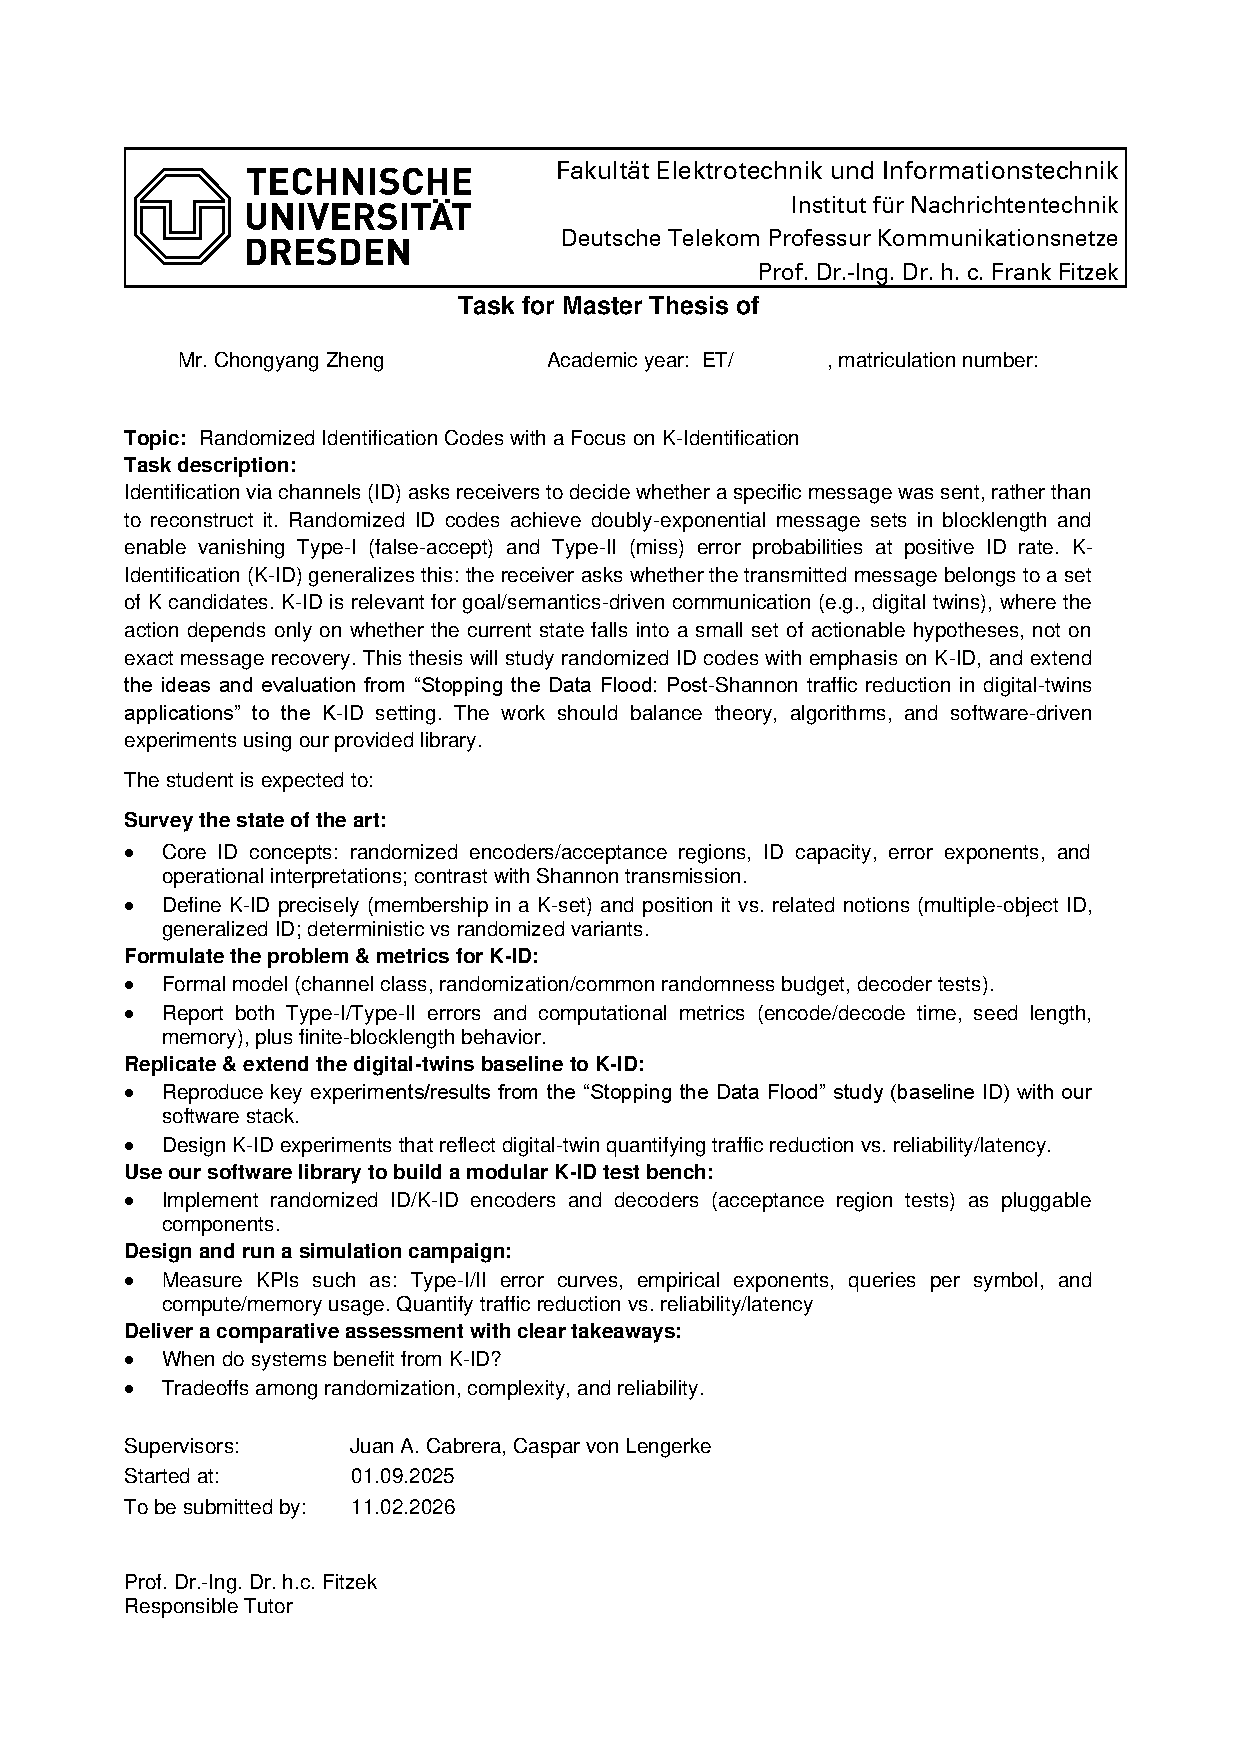
\includepdf[pages=-,pagecommand={}]{Task_Description_Chongyang_Zheng}
\bookmark[page=2]{Task Description Chongyang Zheng}
% ===============================================
%	Confirmation
% ===============================================
% The following uses TUD-specific macros; comment out for now.
\confirmation[supporter=Juan A. Cabrera\and Caspar von Lengerke,pagestyle=empty.tudheadings]
\bookmark[page=3]{Selbstständigkeitserklärung}
% ===============================================
% Abstract (omitted temporarily: uses TUD-specific macros)
% ===============================================
% !TEX root = thesis.tex
% ===============================================
% ===============================================
%	Abstract in german and english
% ===============================================
% ===============================================
\TUDoption{abstract}{multiple,section,notoc}
\renewcaptionname{english}{\abstractname}{Abstract}
\begin{abstract}[pagestyle=empty.tudheadings]%

Identification via channels (ID) asks a receiver to decide whether a specific hypothesis about the transmitted message is true, rather than reconstructing the message itself. This document provides precise definitions, key capacity results, error metrics, and an experimental plan tailored to K-Identification (K-ID), where the receiver asks whether the message belongs to a set of \(K\) candidates. It contrasts randomized vs.\ deterministic (DI) variants, formulates problem and metrics, and outlines a modular test bench and simulation campaign aligned with the provided software stack.

    
\end{abstract}

%\bookmark[page=4]{Kurzfassung/Abstract}

\pagenumbering{Roman} % Roman numbering for the PDF starting with I
% ===============================================
%	Table of contents
% ===============================================
\tableofcontents
\clearpage
% ===============================================
%	Table of figures
% ===============================================
\listoffigures
\clearpage
% ===============================================
%	Table of tables
% ===============================================
\listoftables
% Removed explicit page break to avoid an empty page between LoT and Acronyms
% ===============================================
%	Table of listings
% ===============================================
%
% ===============================================
%	Table of acronyms
% ===============================================
% \glsaddall
% Avoid a forced right-hand start for this front-matter chapter
\begingroup
\KOMAoptions{open=any}
\printacronyms[style=acrotabularx,title={Acronyms}]
\endgroup
\clearpage

\pagenumbering{arabic} % arabic numbering for the PDF starting with 1
% ===============================================
%	Start of mainmatter - chapter 1 and so on...
% ===============================================
% examples chapter removed
\chapter{Introduction}
\label{ch:introduction}

\section{Background and Motivation}
\label{sec:background_motivation}

\glspl{dt} have become a standard component in modern industrial automation for connecting physical assets with their virtual counterparts. By maintaining accurate virtual copies of systems like industrial robots, \glspl{dt} enable real-time monitoring, predictive maintenance, and remote control. In time-critical \gls{cps} applications, the utility of a \gls{dt} is strictly defined by the synchronization accuracy between the physical robot and the digital model~\cite{9013428}. Consequently, ensuring state consistency typically demands \gls{urllc} capabilities to support high-frequency updates.

However, achieving this synchronization through standard periodic transmission is often inefficient in bandwidth-constrained environments. In many control architectures, the \gls{dt} acts as a global supervisor that maintains a high-fidelity state estimate. When the \gls{dt} transmits full state updates to the robot at every time step, it results in significant data redundancy. Since the robot already possesses local sensors to maintain a short-term estimate, "blindly" broadcasting the entire state vector from the \gls{dt} consumes scarce network resources without providing new actionable information. This mismatch between the \gls{dt}'s global knowledge and the robot's local perception creates an opportunity to replace continuous payload reconstruction with sparse, verification-based communication.

To mitigate this redundancy, recent research proposes identification-based \gls{id} synchronization~\cite{9789759}. Unlike classical Shannon-type communication, which aims to reconstruct the full message, \gls{id} schemes focus on a verification task: confirming whether the remote state matches a local hypothesis. Building on this concept, prior works~\cite{fi16030078} demonstrate that transmitting a compressed ``verifier'' (e.g., a short hash or randomized code) instead of the full state can significantly reduce communication traffic. This aligns with semantic communication in \gls{sixg} networks~\cite{doi:https://doi.org/10.1002/9781119765554.ch16}, shifting the focus from what data is sent to what value the data holds for control.

In real-time control loops, deploying \gls{id} synchronization exposes two engineering trade-offs that motivate this thesis. First, the computational overhead of encoding on edge devices may offset the time saved by reducing transmission traffic. This shift from a communication-bound to a computation-bound bottleneck calls for an end-to-end latency analysis that accounts for both compute and communication. Second, reliability becomes a primary concern when moving from exact to semantic verification. In practice, enforcing bitwise synchronization (standard \gls{id}) can be overly conservative, triggering unnecessary updates for benign deviations such as sensor noise. This motivates semantic verification over ``safety sets'', i.e., \gls{kid}. However, the relaxation introduces collision risks, specifically Type~II (miss) errors, where unsafe desynchronizations are incorrectly classified as admissible.

\section{Problem Statement}
\label{sec:problem_statement}

Existing research on \gls{id} has primarily focused on information-theoretic capacity or simple traffic suppression, lacking a comprehensive evaluation of latency, physical safety, and computational feasibility. Specifically, it remains unclear under what bandwidth and computational constraints \gls{id} truly outperforms traditional transmission, and how to quantify the Pareto trade-off between semantic tolerance and safety risk in \gls{kid} systems.

Moreover, semantic tolerance introduces structural constraints that are not visible in purely static formulations: as the acceptance set grows with tolerance, the finite verifier space $2^{n_{ver}}$ can become too small to distinguish all tolerated states, imposing a feasibility limit on the achievable miss probability. Characterizing these feasibility limits and their implications in dynamic settings is part of the open problem addressed in this thesis.

\section{Contributions}
\label{sec:contributions}

To address these limitations, this thesis proposes a comprehensive framework ranging from theoretical modeling to dynamic evaluation, investigating not only the static identification problem but also error evolution in dynamic environments.

First, we develop an end-to-end latency model combining computational and transmission delays to compare algebraic coding (\gls{rsid}) and truncated hashing based on \glsentryshort{sha}-256. For the evaluated software stack, truncated \glsentryshort{sha}-256 achieves low and largely payload-independent encoding latency, while \gls{rsid} incurs higher computation that depends on payload symbolization. These results quantify a practical compute--communication trade-off for edge deployments, while also motivating \gls{rsid} for safety-critical deployments requiring rigorous mathematical guarantees (e.g., provable upper bounds under stated assumptions) on worst-case error-detection failure probability.

Second, we generalize identification to \gls{kid}, introducing semantic tolerance to filter benign jitter. Through parameter sweeps, we map the risk--speedup Pareto frontier and show that moderate tolerance can substantially reduce fallback frequency while keeping safety risks bounded. The analysis also indicates a knee point where additional tolerance yields diminishing speedup while reducing verifier selectivity.

Third, the evaluation is extended to a time-correlated random-walk drift model to capture risks that static analysis may overlook. The results demonstrate that verifiers with insufficient bit-depth (e.g., $n_{ver}=8$) can transform isolated collisions into persistent, undetected boundary breaches once the state drifts beyond the tolerance $R$. To quantify synchronization throughput, we analyze full-state recovery timing via the \gls{sri}. The dynamic results separate the roles of the parameters: $R$ mainly determines how often boundary crossings trigger recovery attempts (updates become sparser as $R$ increases), while $n_{ver}$ determines how often a triggered recovery is missed due to collisions.

\section{Thesis Organization}
\label{sec:organization}

The remainder of this thesis is organized as follows. Chapter~\ref{ch:background} reviews related work, covering the transition from data reconstruction to semantic identification, the mathematical principles of encoding mechanisms, and the control-theoretic background. Chapter~\ref{ch:design_methodology} details the system model, data flow design, and the derivation of theoretical error bounds for \gls{kid}. Chapter~\ref{sec:implementation} describes the implementation of the modular Python simulation framework and the experimental design strategy. Chapter~\ref{sec:results_and_evaluation} presents the experimental results, including latency sensitivity analysis, Pareto optimization of \gls{kid}, and risk assessment under dynamic drift scenarios. Finally, Chapter~\ref{sec:conclusion_and_future_work} concludes the thesis and outlines future research directions.
\chapter{Background and Related Work}
\label{ch:background}

This chapter reviews the transition from classical data transmission to identification-based synchronization, positioning it within the broader context of semantic communication~\cite{zhang2025semantic} for 6G networks. We analyze alternative synchronization strategies—such as differential encoding and event-triggered control—to motivate the engineering need for the identification (\gls{id}) paradigm. We then compare practical encoding mechanisms by contrasting the avalanche dynamics of cryptographic hashing with the geometric properties of algebraic coding. Finally, we discuss how this paradigm generalizes to \gls{kid}, where strict equality constraints are relaxed to semantic safety sets to accommodate natural variability in physical control loops.

% ==================================================================================
% Section 2.1: Macro background (semantic communication and 6G)
% ==================================================================================
\section{From Data Reconstruction to Semantic Identification}
\label{sec:semantic_shift}

In time-critical control loops, the utility of a \gls{dt} depends on its synchronization with the physical asset. Conventional protocols treat this as a data reconstruction problem, where the robot periodically transmits its full state vector $S_t$ (e.g., joint angles and velocities) to the \gls{dt}. While robust, this approach overlooks a key redundancy: the \gls{dt}, using its internal kinematic model, already maintains a prediction $\hat{S}_t$ of the robot's state. The communication task is therefore not to inform the \gls{dt} ``where the robot is,'' but to verify ``whether the \gls{dt}'s prediction is correct.''

This shift aligns with the paradigm of semantic communication~\cite{strinati2024goal} in 6G networks. Unlike classical Shannon-type communication, which emphasizes accurate reconstruction, semantic communication emphasizes information that matters for the receiver's goal. In the context of \gls{urllc}, this suggests prioritizing ``actionable'' information—such as safety violations—over raw telemetry.

Accordingly, the coding objective shifts from Shannon's transmission capacity to the identification capacity defined by Ahlswede and Dueck~\cite{ahlswede1989}. In transmission, each possible state must map to a disjoint decoding set, limiting the number of distinguishable states to $2^{nR}$ for blocklength $n$. In contrast, identification permits overlaps between decoding sets, as long as pairwise intersections are statistically negligible. This relaxation enables a doubly exponential growth in identifiable states ($2^{2^{nR}}$), meaning that short verifiers can discriminate among an extremely large state space while allowing a vanishingly small error probability.

% ==================================================================================
% Section 2.2: Alternative strategies
% ==================================================================================
\section{Alternative Synchronization Strategies}
\label{sec:alternatives}

Before detailing the implementation of identification, it is necessary to rigorously evaluate why established data reduction strategies—specifically Delta Encoding and Event-Triggered Control—are often insufficient for unreliable edge networks.

\subsection{Full State Transmission (The Baseline)}
The standard baseline in industrial automation is the periodic transmission of the full state vector $S_t$. This approach is favored for its statelessness; each packet is self-contained. If a packet at time $t$ is lost due to channel interference, the packet at $t+1$ allows the \gls{dt} to immediately recover the correct state. However, this robustness comes at the cost of extreme bandwidth inefficiency. In steady-state operations, where $S_t \approx S_{t-1}$, the information entropy of the transmitted packet is near zero, yet it consumes the full bandwidth allocated to the payload $n_{data}$.

\subsection{Delta Encoding and the Drift Problem}
To address this redundancy, Delta Encoding~\cite{mogul1997potential} (or differential transmission) is frequently employed. This method transmits only the difference vector $\Delta_t = S_t - S_{t-1}$. Since $\Delta_t$ typically has a smaller dynamic range than the absolute state $S_t$, it can be quantized with fewer bits, offering significant compression ratios.

However, Delta Encoding introduces a key vulnerability: statefulness. The reconstruction of the current state at the receiver, denoted as $S'_t$, depends recursively on the history of received updates: $S'_t = S'_{t-1} + \Delta_t$. This recursive dependency creates a clear failure mode in unreliable transport protocols like \gls{udp}. A single lost packet $\Delta_k$ causes a persistent offset between the physical robot and the \gls{dt}, a phenomenon known as ``state drift.''~\cite{ishibashi2007lag} While reliable protocols like \gls{tcp} can prevent packet loss, retransmissions introduce non-deterministic latency jitter, which can violate the timing deadlines of real-time control loops. Therefore, Delta Encoding poses a high risk for \gls{urllc} applications.

\subsection{Event-Triggered Control (ETC)}
Another prominent alternative is Event-Triggered Control (\gls{etc}). Unlike Time-Triggered (periodic) systems, \gls{etc} only transmits data when the deviation between the current state and the last transmitted state exceeds a threshold $\delta$: $\|S_t - S_{last\_sent}\| > \delta$~\cite{tabuada2007event}. This approach effectively silences the network during periods of inactivity.

Nevertheless, \gls{etc} relies fundamentally on a ``push'' communication model. A silent channel is ambiguous to the receiver: it could indicate that the system is operating safely within bounds, or it could indicate that the sensor has failed or the link has been severed. In safety-critical robotics, such ambiguity is often unacceptable. Furthermore, \gls{etc} requires the sensing node to perform continuous monitoring and threshold checking, pushing computational complexity to the energy-constrained edge~\cite{heemels2012introduction}.

\subsection{The Identification Advantage}
In contrast to these alternatives, the \gls{id} scheme proposed in this thesis combines statelessness with strong compression. Unlike Delta Encoding, \gls{id} verification checks the absolute state $S_t$ directly and is therefore immune to drift; if a packet is lost, the next packet again provides an independent check. Unlike \gls{etc}, \gls{id} supports a ``verify'' model, allowing the \gls{dt} to actively confirm synchronization with minimal overhead. This combination is well-suited for maintaining high-fidelity \glspl{dt} over unreliable networks.

% ==================================================================================
% Section 2.3: Encoding mechanisms
% ==================================================================================
% ==================================================================================
% Section 2.3: 编码机制深化 (Hardcore Math Version)
% ==================================================================================
\section{Encoding Mechanisms: Mathematical Structure and Bias}
\label{sec:encoding_mechanisms}

To realize the theoretical capacity of identification in edge computing, the encoding process must map a high-dimensional state space $\mathcal{S}$ into a low-dimensional verifier space $\mathcal{V}$ while minimizing collision probabilities. This section dissects the internal mechanisms of the two candidate algorithms—cryptographic hashing (SHA-256) and algebraic coding (RS-ID)—to reveal the mathematical origins of their reliability.

\subsection{Cryptographic Construction: The SHA-256 Architecture}
\label{subsec:sha256_structure}

To understand the source of the high entropy in the generated verifiers, it is necessary to examine the internal structure of the SHA-256 algorithm~\cite{nist2015secure}. SHA-256 belongs to the SHA-2 family and is built upon the Merkle-Damgård construction, which iteratively processes the input state $S$ using a dedicated compression function. The process consists of three mathematically distinct stages: preprocessing, message expansion, and the state update loop.

\subsubsection{Preprocessing and Padding}
The input message $M$ (comprising the state $S$ concatenated with the seed $r$) is first padded to ensure its length is a multiple of 512 bits. The padding scheme appends a single '1' bit, followed by $k$ zero bits, and finally a 64-bit integer representing the original message length. This padded message is parsed into $N$ blocks of 512 bits, denoted as $M^{(1)}, M^{(2)}, \dots, M^{(N)}$.

\subsubsection{Message Schedule (Expansion)}
The core of the diffusion process begins with the Message Schedule. Each 512-bit block $M^{(i)}$ is expanded from 16 words (32-bit each) into 64 words, denoted as $W_0, \dots, W_{63}$.
The first 16 words are copied directly from the message block. The remaining 48 words are generated recursively, creating a complex dependency chain where every future bit depends on multiple past bits:
\begin{equation}
    W_t = \sigma_1(W_{t-2}) + W_{t-7} + \sigma_0(W_{t-15}) + W_{t-16} \pmod{2^{32}}
\end{equation}
where the small sigma functions $\sigma_0$ and $\sigma_1$ introduce the initial bitwise diffusion via rotation (ROTR) and shifting (SHR):
\begin{align}
    \sigma_0(x) &= ROTR^{7}(x) \oplus ROTR^{18}(x) \oplus SHR^{3}(x) \\
    \sigma_1(x) &= ROTR^{17}(x) \oplus ROTR^{19}(x) \oplus SHR^{10}(x)
\end{align}
This expansion ensures that a single bit flip in the input $M^{(i)}$ propagates to affect a vast majority of the 64 words in the schedule, setting the stage for the avalanche effect.

\subsubsection{The Compression Loop}
The 64 expanded words $W_t$ are then fed into the compression function. The working state consists of eight 32-bit variables, labeled $a$ through $h$, initialized to constant prime-root values. For each step $t$ from 0 to 63, the state is updated using two temporary variables $T_1$ and $T_2$:
\begin{align}
    T_1 &= h + \Sigma_1(e) + Ch(e, f, g) + K_t + W_t \\
    T_2 &= \Sigma_0(a) + Maj(a, b, c)
\end{align}
Here, $K_t$ represents 64 constant 32-bit words. The non-linear logical functions $Ch$ (Choose) and $Maj$ (Majority), along with the big sigma functions $\Sigma_0$ and $\Sigma_1$, serve as the mixing engine:

\begin{align}
    Ch(x, y, z) &= (x \land y) \oplus (\neg x \land z) \\
    Maj(x, y, z) &= (x \land y) \oplus (x \land z) \oplus (y \land z) \\
    \Sigma_0(x) &= ROTR^{2}(x) \oplus ROTR^{13}(x) \oplus ROTR^{22}(x) \\
    \Sigma_1(x) &= ROTR^{6}(x) \oplus ROTR^{11}(x) \oplus ROTR^{25}(x)
\end{align}
After calculating $T_1$ and $T_2$, the registers are shifted ($h \leftarrow g, g \leftarrow f, \dots$), and updated as:
\begin{equation}
    e \leftarrow d + T_1, \quad a \leftarrow T_1 + T_2
\end{equation}
This rigorous mixing guarantees that after 64 rounds, every bit of the final hash output is a complex, non-linear function of every bit of the input block. Finally, the output verifier $v$ is obtained by truncating this digest to the target length $n_{ver}$, retaining the high-entropy properties generated by this procedure.


\subsection{Algebraic Construction: The Geometry of RS-ID}
\label{subsec:rsid_geometry}
In contrast to the bitwise diffusion of SHA-256, \gls{rsid} relies on the geometric properties of polynomials over finite fields\cite{schwartz1980fast}. 

\subsubsection{Data as a Polynomial Curve}
Let the state vector $S$ be decomposed into $k$ segments $\{s_0, s_1, \dots, s_{k-1}\}$, where each segment is an element of the Galois Field $\mathbb{F}_q$. We interpret these segments not as raw data, but as coefficients of a unique polynomial curve $P_S(x)$ of degree $k-1$:
\begin{equation}
    P_S(x) = s_0 + s_1 x + s_2 x^2 + \dots + s_{k-1} x^{k-1} = \sum_{i=0}^{k-1} s_i x^i
\end{equation}
The generation of a verifier $v$ using a random seed $r$ is geometrically equivalent to sampling this curve at the coordinate $x=r$:
\begin{equation}
    v = P_S(r) \pmod q
\end{equation}


\subsubsection{Collision as Intersection}
A collision (Type II error) occurs when the true state $S$ and the predicted state $\hat{S}$ are distinct ($S \neq \hat{S}$), yet their verifiers match ($v = \hat{v}$). In our geometric model, this implies:
\begin{equation}
    P_S(r) = P_{\hat{S}}(r) \implies P_S(r) - P_{\hat{S}}(r) = 0
\end{equation}
Let $\Delta(x) = P_S(x) - P_{\hat{S}}(x)$ be the difference polynomial. Since $S \neq \hat{S}$, $\Delta(x)$ is a non-zero polynomial with degree at most $k-1$. By the Fundamental Theorem of Algebra, a non-zero polynomial of degree $d$ can have at most $d$ roots. 

This geometric constraint provides the rigorous upper bound for the collision probability. The number of "bad seeds" $r$ that cause a collision is limited to the number of intersection points between the two curves $P_S(x)$ and $P_{\hat{S}}(x)$, which is at most $k-1$. Thus, for a field of size $q$, the probability is:
\begin{equation}
    P_{miss} = \frac{\text{Number of Roots}}{q} \le \frac{k-1}{q}
\end{equation}
This derivation visualizes the identification process as "checking for intersection." Since two distinct curves cannot intersect everywhere, checking a random point $r$ effectively distinguishes them with high probability~\cite{schwartz1980fast}.

\subsection{Structural Blindness and Randomization}
A critical limitation of deterministic compression is ``structural blindness.'' Consider a simplified case where the encoder uses a modulo operation. If the error $e = S - \hat{S}$ happens to be a multiple of the modulus, the generated verifiers will be identical ($v = \hat{v}$) regardless of the magnitude of the error. Even if the robot's state $S$ changes continuously, this error pattern might persist, leading to a persistent Type II (miss) error.

To eliminate structural blindness, identification theory mandates the use of common randomness---a shared seed $r$ that changes with each transmission. In \gls{rsid}, changing $r$ corresponds to sampling the polynomial at a different $x$-coordinate. In \gls{sha}, appending a time-varying salt ($S || r$) changes the avalanche dynamics. By varying $r$, the mapping changes at every time step; although a collision may occur at a specific seed $r_1$, the probability that the same error causes a collision at a new seed $r_2$ is independent. This converts potential ``permanent failures'' into ``transient probabilistic events.''

% ==================================================================================
% Section 2.4: Common randomness
% ==================================================================================
\section{Operational Prerequisite: Common Randomness Generation}
\label{sec:common_randomness}

As established in Section~\ref{sec:encoding_mechanisms}, the theoretical validity of identification codes hinges on the availability of \gls{cr}---a shared source of entropy between the encoder (robot) and the decoder (\gls{dt}). Without a dynamic shared seed $r$, the system reduces to a deterministic mapping and becomes susceptible to structural blindness, where persistent error patterns can remain undetectable~\cite{9789759}. Therefore, the practical deployment of \gls{id} requires a robust mechanism to generate or synchronize $r$ without negating the bandwidth savings.

The most straightforward approach to establish this shared entropy is to use synchronized \glspl{prng}, formally standardized as \glspl{drbg}~\cite{nist80090a}. By initializing identical generators with a pre-shared secret key and tying them to a synchronized time index---typically maintained via the \gls{ptp}~\cite{ieee1588}---both the robot and the \gls{dt} can locally derive an identical sequence of seeds $r_t$ for each time slot. While this method has zero communication overhead during steady-state operation, it introduces a dependency on clock synchronization. Any drift in the robot's clock relative to the \gls{dt} results in a seed mismatch ($r_{robot} \neq r_{DT}$), causing verifier checks to fail continuously. This loss of synchronization can manifest as a sustained burst of false positives, forcing the system into a fallback mode until resynchronization.

Alternative approaches, such as \gls{plkg}, attempt to extract randomness from channel reciprocity in wireless networks~\cite{li2019physical}. While \gls{plkg} aligns with physical-layer security paradigms by exploiting channel noise entropy~\cite{ahlswede1998common}, it often requires additional reconciliation overhead to correct quantization mismatches. Consequently, to isolate the performance characteristics of the encoding mechanisms, this thesis assumes an idealized PRNG-based synchronization model for the experimental evaluation.

% ==================================================================================
% Section 2.5: Theoretical limits and trade-offs
% ==================================================================================
\section{Theoretical Limits and Algorithmic Trade-offs}
\label{sec:theoretical_limits}

While the introduction of randomization allows for drastic compression, the output length cannot be reduced arbitrarily. The choice between algebraic (RS-ID) and cryptographic (SHA-256) implementations is governed by a fundamental tension between theoretical error bounds and computational efficiency.

\subsection{The Algebraic Limit: Saturation and Field Size}
In the polynomial model of \gls{rsid}, the verifier length $L$ is constrained by the algebraic properties of the state representation. Since a state vector of length $k$ is interpreted as a polynomial of degree $k-1$, two distinct state polynomials can intersect at most at $k-1$ points. To ensure reliable identification, the size of the evaluation field $Q = 2^L$ must be significantly larger than the number of potential intersection points. If $Q < k$, the ``collision points'' can saturate the field, making it mathematically impossible to find a seed $r$ that distinguishes the two states via a single sample.

Therefore, a necessary condition for the reliability of algebraic identification is that the field size must grow with the data size:
\begin{equation}
    2^L > k \quad \Rightarrow \quad L > \log_2 k
\end{equation}
This inequality represents the physical manifestation of the double exponential limit established by Ahlswede and Dueck~\cite{ahlswede1989}. It dictates that for \gls{rsid}, the verifier length $L$ must scale logarithmically with the data size $k$. As long as this condition is met, \gls{rsid} provides a rigorous upper bound $\lambda_2$ on the collision probability, ensuring that no pair of states exceeds a worst-case error threshold regardless of the input distribution~\cite{9789759}.

\subsection{The Cryptographic Perspective: Independence from Data Size}
In contrast to the algebraic constraints, cryptographic methods like \gls{sha} operate under the Random Oracle Model. The collision probability of a truncated hash is approximately $2^{-L}$, which is invariant to the input data size $k$. Unlike \gls{rsid}, \gls{sha} does not suffer from ``saturation'' when the input data grows. A 16-bit hash verifier has the same uniform collision probability whether verifying a 100-byte state or a 1-megabyte state. This makes cryptographic approaches robust for large-scale data vectors where satisfying $2^L > k$ might require an impractically large field for \gls{rsid}.

\subsection{Engineering Trade-offs: Bound vs. Speed}
\label{subsec:tradeoffs}

From a safety-critical perspective, the algebraic structure of \gls{rsid} provides a deterministic guarantee. Based on the Fundamental Theorem of Algebra, the number of collision-causing seeds for a message of length $k$ is bounded by the polynomial degree $k-1$~\cite{9789759}. This yields the following worst-case bound on the miss probability:
\begin{equation}
    P_{miss} \le \frac{k-1}{q}
\end{equation}
where $q$ is the field size. Such a worst-case guarantee is relevant for mission-critical control loops in which adversarial or pathological error distributions must be handled analytically rather than statistically.

The same bound also highlights a scalability limitation: the number of potentially colliding seeds grows linearly with data size ($P_{miss} \propto k$). For large payloads (e.g., LiDAR or vision streams), preserving a small upper bound requires increasing $q$, which in turn increases the latency of finite-field arithmetic. In contrast, cryptographic hashing (e.g., \gls{sha}) is commonly modeled as a random oracle, where a truncated verifier of length $L$ yields a collision probability on the order of $2^{-L}$ that does not depend on $k$. This makes hash-based approaches attractive when the payload size dominates system constraints.

Accordingly, this thesis evaluates both mechanisms to cover the spectrum of edge computing requirements: \gls{rsid} is used as a theoretical reference for lightweight control signals (small $n_{data}$), while \gls{sha} is used to demonstrate computational scalability for data-intensive applications (large $n_{data}$).


% ==================================================================================
% Section 2.6: K-ID
% ==================================================================================
\section{Semantic Verification: Adapting to Control Flexibility}
\label{sec:kid_application}

While standard identification provides a rigorous method for exact state verification, its binary nature—accepting only a single, precise value—often contradicts the operational flexibility required in modern robotic control. In many practical scenarios, the \gls{dt} does not need to enforce a strict equality constraint ($x = \hat{x}$) but rather needs to guarantee that the robot operates within a permissible semantic range. This nuance necessitates the adoption of \gls{kid}, which generalizes the verification target from a unique point to a semantic safety set.

\subsection{The Autonomous Driving Scenario}
Consider a practical example of an autonomous robot (or vehicle) navigating a public roadway. The control policy might specify a safe velocity corridor, such as ``maintain speed between 40 km/h and 60 km/h.'' If the robot moves at 45 km/h while the \gls{dt} predicted 50 km/h, a standard \gls{id} scheme would flag this as a collision (mismatch) because the hashed values of ``45'' and ``50'' are distinct. This triggers an unnecessary data transmission to correct a behavior that is semantically valid.

\gls{kid} resolves this inefficiency by defining the acceptance region $\mathcal{B}$ as the interval $[40, 60]$. As long as the robot's state falls within this set, the \gls{kid} verifier confirms validity without consuming bandwidth for minor deviations.

\subsection{Human-Robot Collaboration and Jitter}
This logic extends beyond simple velocity constraints to more complex spatial and interactive scenarios. For instance, in \gls{hrc}, the exact coordinates of a robotic arm are less critical than ensuring the end-effector remains outside a defined ``human safety bubble''~\cite{9013428}. Similarly, for high-precision assembly tasks involving compliant mechanisms, the robot may exhibit minor high-frequency vibrations (jitter) that are mechanically acceptable. Standard \gls{id} would treat these micro-vibrations as errors, whereas \gls{kid} can be tuned to ignore high-frequency noise while still detecting significant trajectory deviations.

By shifting the verification paradigm from data exactness to semantic compliance, \gls{kid} aligns the synchronization protocol with the actual control objectives. It allows the system to filter out benign variability—whether it be speed fluctuations, sensor noise, or compliant jitter—and focus limited communication resources on detecting genuine safety violations. This thesis specifically investigates the implementation of such semantic verification using randomized encoding on edge constraints.

\subsection{Discussion: Trading Freshness for Value}
\label{subsec:aoi_voi_tradeoff}

The scenarios described above illustrate a deviation from traditional network optimization. Conventional real-time protocols often aim to minimize the \gls{aoi}~\cite{kaul2012real}, keeping the \gls{dt}'s estimate as fresh as possible regardless of content. Under an \gls{aoi}-minimization strategy, the robot would transmit its velocity continuously even when cruising steadily within the safe corridor, purely to prevent the timestamp from ``aging.''

\gls{kid} challenges this paradigm by introducing a semantic filter that prioritizes the \gls{voi} over simple freshness. As demonstrated in the autonomous driving case, a ``stale'' position estimate (high \gls{aoi}) that remains within the safety tolerance $\mathcal{B}$ retains its utility for the control loop. By allowing \gls{aoi} to increase during semantically safe intervals, \gls{kid} trades unnecessary freshness for bandwidth efficiency. This is consistent with goal-oriented communication~\cite{strinati2024goal}, where the objective shifts from minimizing average latency to minimizing the latency of meaningful (unsafe) updates.

% ==================================================================================
% Section 2.7: Control-theoretic perspectives
% ==================================================================================
\section{Control-Theoretic Perspectives: Deadbands and Stability}
\label{sec:control_theory}

Beyond communication efficiency, the deployment of \gls{kid} changes the control loop structure. From a control-theoretic perspective, \gls{kid} yields a \gls{ncs} operating under a semantic sampling policy. This section analyzes the implications for stability and execution semantics, and maps \gls{kid} parameters to established control concepts.

\subsection{K-ID as Deadband Control}
The tolerance mechanism in \gls{kid}, defined by the acceptance set $\mathcal{B}$, is mathematically equivalent to Deadband Control (or Dead-Zone Control) in non-linear systems theory. In classical mechanics, deadbands are often viewed as parasitic nonlinearities (e.g., gear backlash) that degrade performance. However, in resource-constrained \gls{ncs}, artificially introduced deadbands are a recognized strategy for reducing actuator wear and communication load~\cite{astrom2002comparison}.

By enforcing a ``silence'' policy when the synchronization error $e_t = S_t - \hat{S}_t$ satisfies $|e_t| \le K$, \gls{kid} implements Lebesgue Sampling (sampling based on value domains), as opposed to the traditional Riemann Sampling (sampling based on time domains). This semantic filtering prevents the control loop from reacting to high-frequency, low-amplitude noise (chattering), thereby reducing mechanical stress on physical actuators while preserving bandwidth for significant trajectory corrections.

\subsection{Prevention of Zeno Behavior}
A pervasive challenge in standard Event-Triggered Control (\gls{etc}) is the risk of Zeno behavior---a phenomenon where the inter-event time converges to zero, causing the system to trigger an infinite number of updates in a finite time interval~\cite{heemels2012introduction}. This can occur when the state trajectory ``slides'' along the triggering threshold, potentially leading to computational livelock or network storms.

\gls{kid} inherently circumvents this instability through its hybrid architecture. Although the decision to update is event-driven (based on the semantic check $v \in \mathcal{V}_K$), the verification opportunity occurs at discrete, time-triggered intervals (ticks). This imposes a strict lower bound on the inter-transmission time, denoted as $T_{min} \ge T_{tick}$. By structural design, \gls{kid} guarantees Zeno-freeness, ensuring that the network load remains deterministically bounded even in worst-case divergence scenarios.

\subsection{Bounded-Input Bounded-Output (BIBO) Stability}
The introduction of the semantic tolerance $K$ raises the question of closed-loop stability. Under \gls{kid}, the \gls{dt} (controller) operates on an estimated state $\hat{S}_t$ that deviates from the true plant state $S_t$ by an error term $\delta_t$. Assuming the absence of collision-induced miss errors (which are probabilistically negligible as shown in Section~\ref{sec:encoding_mechanisms}), the synchronization error is strictly bounded:
\begin{equation}
    ||\delta_t|| = ||S_t - \hat{S}_t|| \le K
\end{equation}
From a stability analysis perspective, this bounded error acts as a bounded disturbance input to the controller. According to the principle of \gls{bibo} stability~\cite{hespanha2007survey}, as long as the underlying control law can reject disturbances of magnitude $K$, the closed-loop system remains stable. This implies that the design of $K$ is not only a traffic parameter but also a stability constraint: $K$ must remain within the controller's stability margin (or region of attraction).

\chapter{Design Methodology}
\label{ch:design_methodology}

% \section{Overview}
This chapter formulates the system model for identification-based synchronization and derives the theoretical bounds for its reliability and latency. We contrast the data flow of classical transmission with the proposed identification scheme, explicitly breaking down the operational stages from state generation to synchronization. We then quantify the collision probabilities and end-to-end latency based on these distinct workflows.

\section{System Model and Data Flow}
\label{sec:system_model}

We consider a networked control system where a Robot (Sender) synchronizes its state $S_t$ with a Digital Twin (Receiver) maintaining a prediction $\hat{S}_t$. The fundamental difference between the two approaches lies in their data processing pipelines.

\subsection{Baseline: Traditional Transmission Flow}
The standard synchronization protocol follows a linear, ``always-on'' approach. As illustrated in Figure~\ref{fig:trad_flow}, the data flow consists of three sequential stages:

\begin{figure}[htbp]
    \centering
    % Ensure you have the file 'figures/trad.png'
    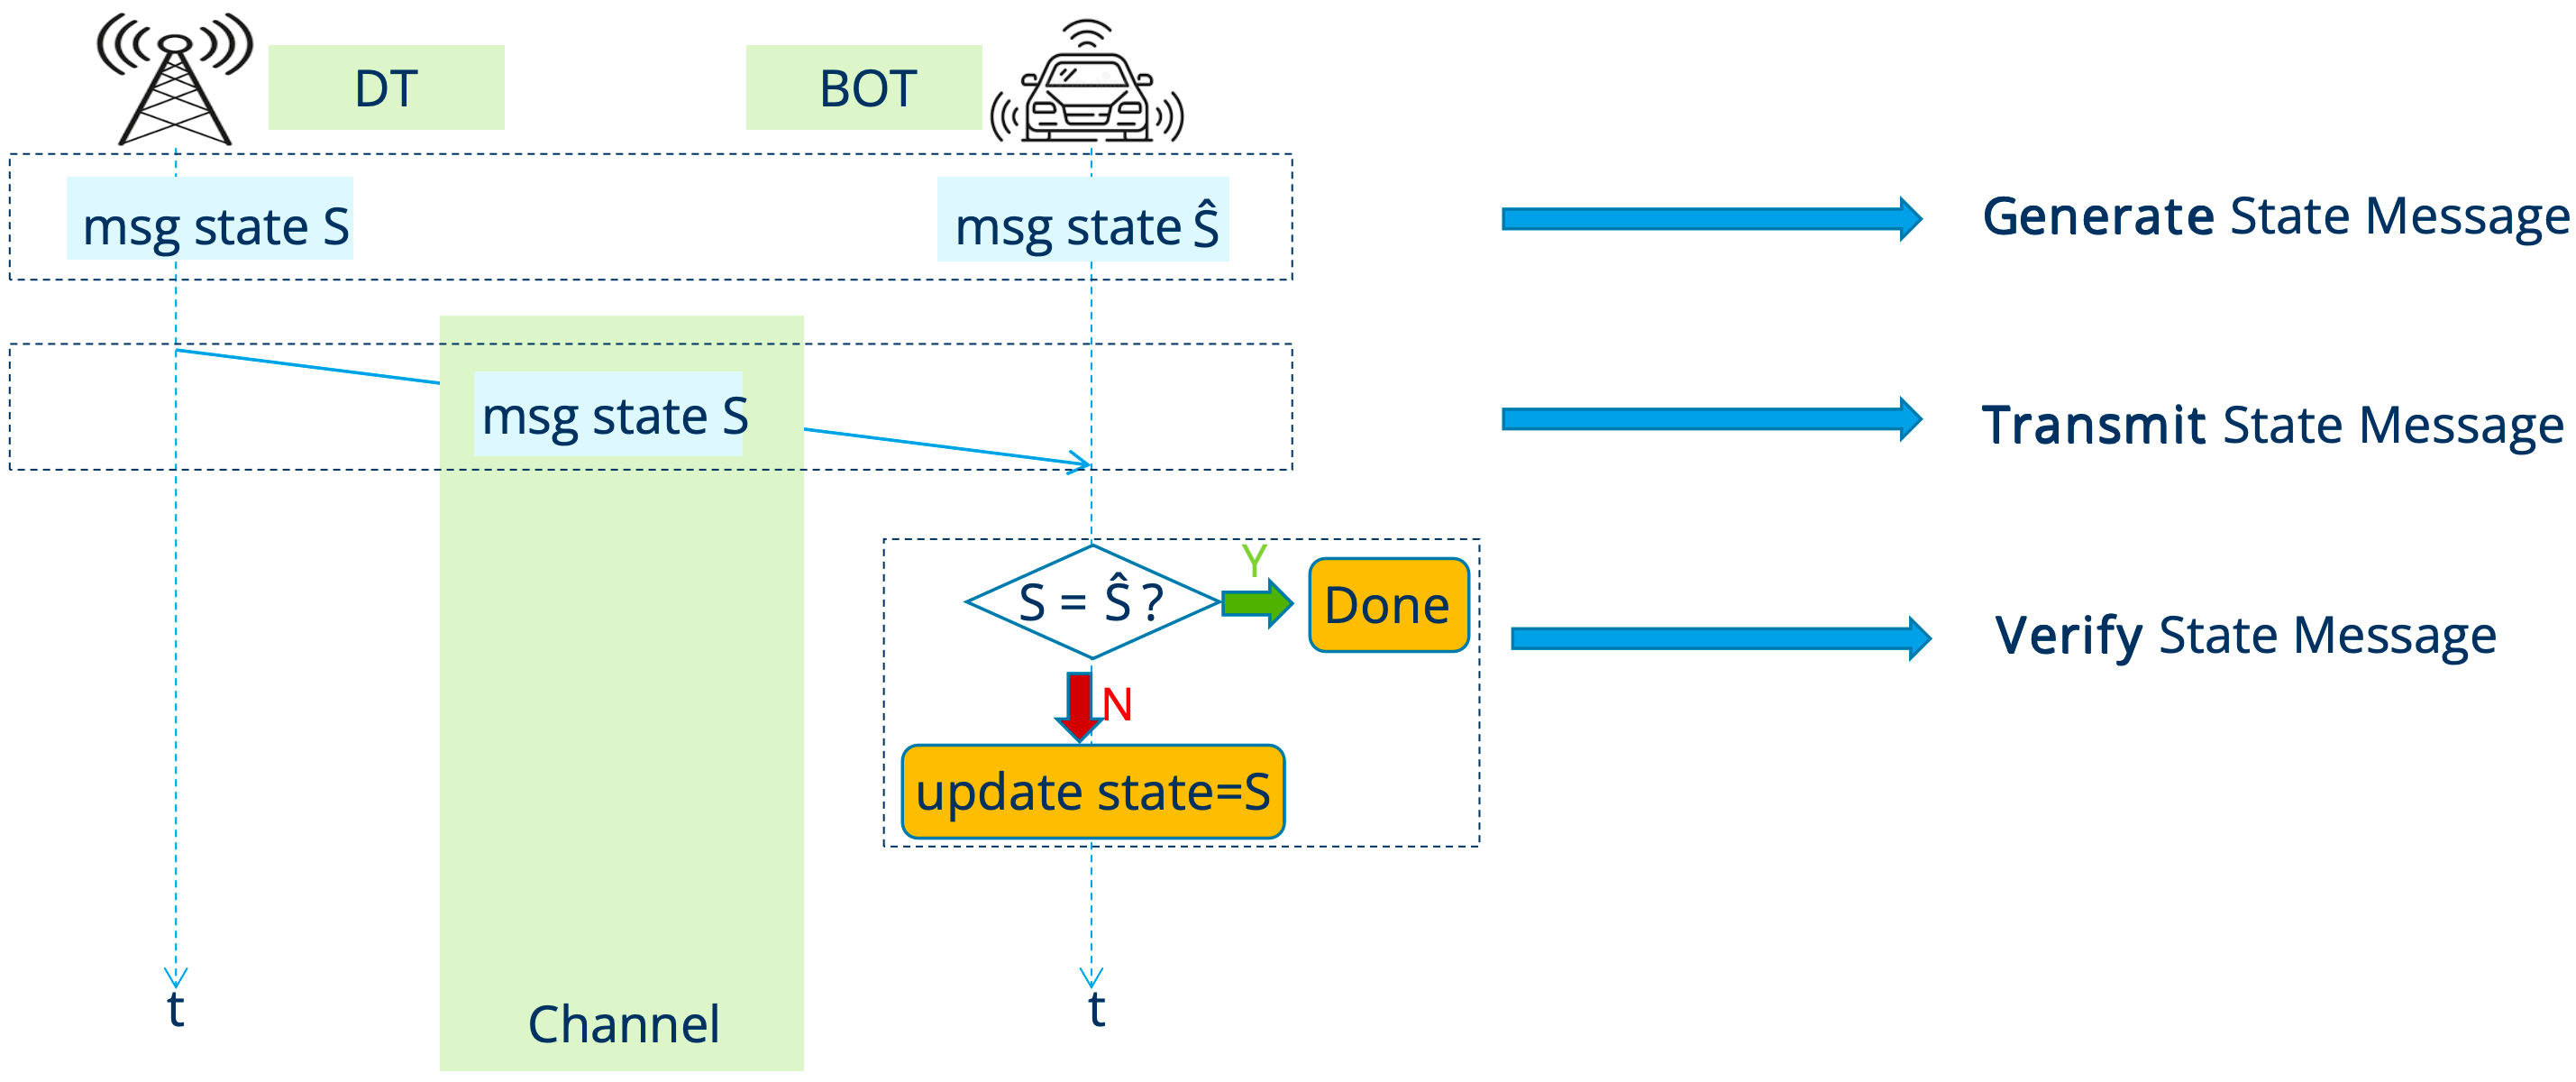
\includegraphics[width=0.8\textwidth]{figures/trad.png}
    \caption{Data flow of Traditional Synchronization: The full state is transmitted regardless of the Digital Twin's knowledge.}
    \label{fig:trad_flow}
\end{figure}

\begin{enumerate}
    \item \textbf{Generate:} The robot samples its sensors to generate the full state message $S_t$ of size $n_{data}$.
    \item \textbf{Transmit:} The entire payload $S_t$ is transmitted over the channel. This step consumes bandwidth proportional to the state dimension, regardless of whether $S_t$ has changed significantly or matches the DT's prediction.
    \item \textbf{Verify/Update:} The DT receives the message, overwrites its local prediction $\hat{S}_t$ with the received $S_t$, and confirms the update.
\end{enumerate}
This process is robust but inefficient, as the \textbf{Transmit} stage imposes a heavy, constant latency penalty ($T_{trans} = n_{data}/B$).

\subsection{Proposed: Identification (ID) Data Flow}
The identification-based protocol introduces computational intelligence to reduce communication load. As shown in Figure~\ref{fig:id_flow}, the pipeline is expanded to five stages, introducing a ``Verify-then-Correct'' logic:

\begin{figure}[htbp]
    \centering
    % Ensure you have the file 'figures/ID.png'
    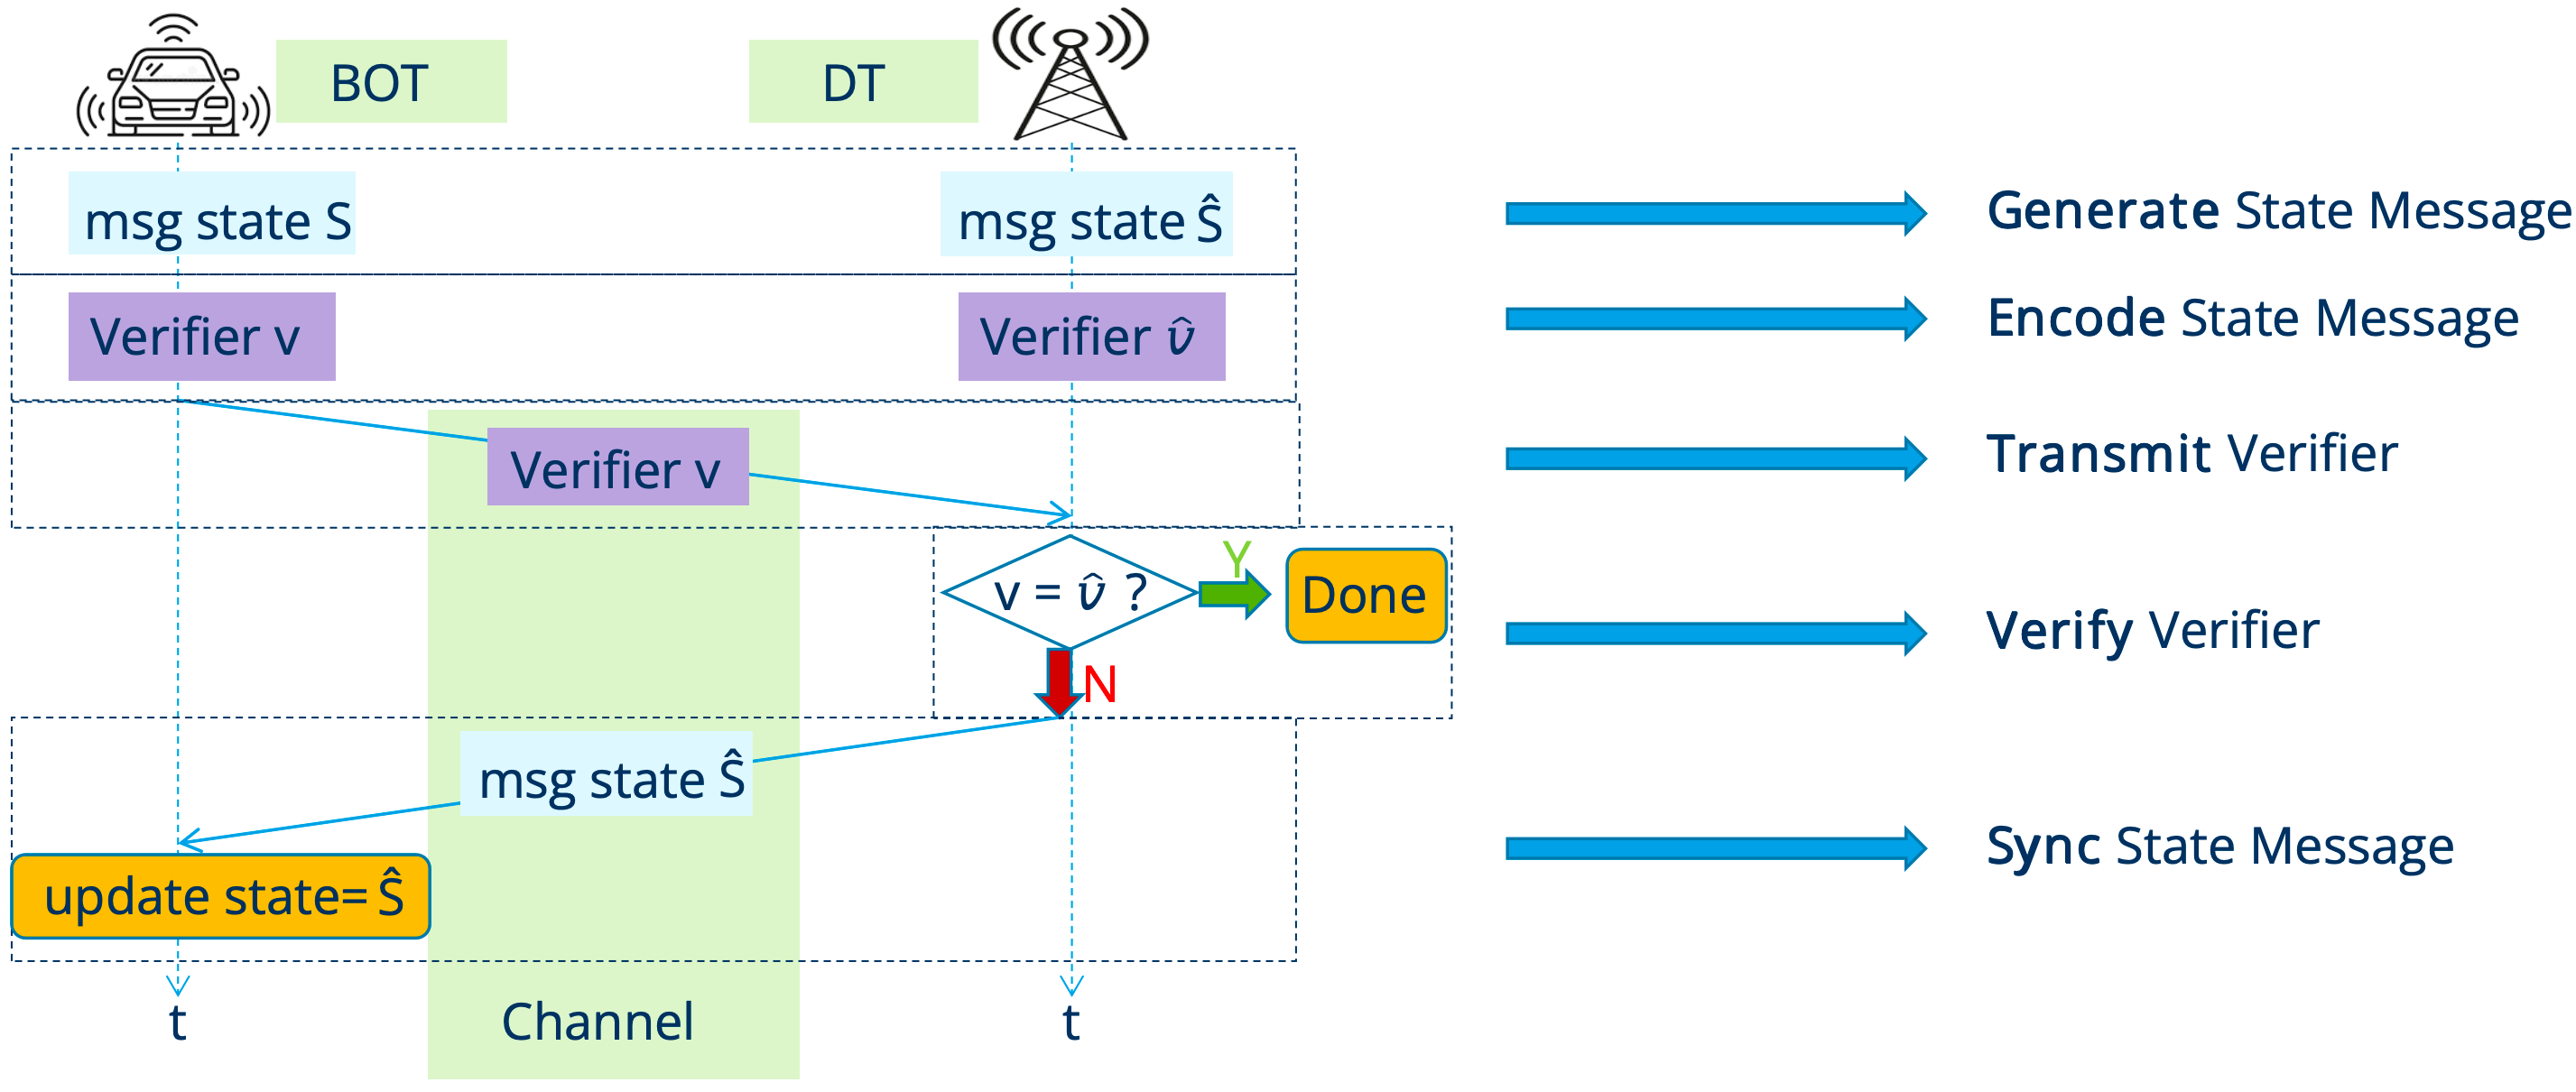
\includegraphics[width=0.8\textwidth]{figures/ID.png}
    \caption{Data flow of ID Synchronization: High-bandwidth transmission is replaced by local encoding and conditional fallback.}
    \label{fig:id_flow}
\end{figure}

\begin{enumerate}
    \item \textbf{Generate:} Both the Robot and the DT independently generate their respective state views: the actual state $S_t$ and the predicted state $\hat{S}_t$.
    \item \textbf{Encode:} Instead of preparing the full message for transmission, the Robot computes a compact signature (verifier) $v = E(S_t, r)$ using a shared seed $r$. Simultaneously, the DT computes its local reference $\hat{v} = E(\hat{S}_t, r)$. This step introduces a computational latency ($t_{ver}$) but drastically compresses the data.
    \item \textbf{Transmit:} Only the short verifier $v$ (size $n_{ver} \ll n_{data}$) is sent over the channel.
    \item \textbf{Verify:} The DT compares the received $v$ with its local $\hat{v}$.
    \item \textbf{Sync (Conditional):} 
    \begin{itemize}
        \item If $v = \hat{v}$, the process terminates (Done).
        \item If $v \neq \hat{v}$, a mismatch is detected. The system enters a fallback mode, requesting the full transmission of $S_t$ to resynchronize.
    \end{itemize}
\end{enumerate}

\section{Encoding Mechanisms and Reliability Analysis}
\label{sec:reliability_analysis}

The safety of the ID flow depends on the reliability of the \textbf{Verify} stage. A critical failure occurs if the states differ ($S_t \neq \hat{S}_t$) but their verifiers collide ($v = \hat{v}$), defined as a Type II Error ($p_{miss}$). We investigate two distinct encoding mechanisms, detailing their construction and theoretical error bounds.

\subsection{Algebraic Construction and Error Analysis (RS-ID)}
\label{sec:rsid_proof}

The core challenge of the RS-ID scheme is to map a high-dimensional state vector $S$ of length $n_{data}$ into a single element within a finite field $\mathbb{F}_q$, where the field size $q = 2^{n_{ver}}$ is determined by the output bandwidth constraint.

\textbf{Polynomial Construction (The ``Chunking'' Process)}
Since the operations are defined over $\mathbb{F}_{q}$, a state vector $S$ typically exceeds the capacity of a single field element (i.e., $n_{data} \gg n_{ver}$). To resolve this dimensionality mismatch, we decompose the bitstream $S$ into $k$ segments, where each segment represents a coefficient in the field:
\begin{equation}
    k = \left\lceil \frac{n_{data}}{n_{ver}} \right\rceil
\end{equation}
Let $S$ be represented as a vector of coefficients $\{s_0, s_1, \dots, s_{k-1}\}$, where each $s_i \in \mathbb{F}_q$. We then construct a polynomial $P_S(x)$ of degree at most $k-1$:
\begin{equation}
    P_S(x) = \sum_{i=0}^{k-1} s_i x^i
\end{equation}
The verifier $v$ is obtained by evaluating this polynomial at a shared random seed $r$: $v = P_S(r)$.

\textbf{Proof of Collision Probability}
A Type II error (Miss) occurs when the Digital Twin predicts an incorrect state $\hat{S} \neq S$, yet the generated verifiers are identical ($P_{\hat{S}}(r) = P_S(r)$).
We define a \textit{difference polynomial} $\Delta(x)$:
\begin{equation}
    \Delta(x) = P_S(x) - P_{\hat{S}}(x)
\end{equation}
Since $S \neq \hat{S}$, at least one coefficient differs, making $\Delta(x)$ a non-zero polynomial with a degree $\text{deg}(\Delta) \leq k-1$.
A collision event is mathematically equivalent to finding a root of this difference polynomial: $\Delta(r) = 0$.

We invoke the \textbf{Schwartz-Zippel Lemma} (Lemma 1 in~\cite{schwartz1980fast}), which states that a non-zero polynomial of degree $d$ over a field $\mathbb{F}_q$ has at most $d$ roots.
Mapping this theorem to our system parameters:
\begin{itemize}
    \item The polynomial degree $d$ corresponds to the chunk count $k \approx n_{data}/n_{ver}$.
    \item The sample space size corresponds to the field size $q = 2^{n_{ver}}$.
\end{itemize}
Consequently, for a uniformly distributed random seed $r$, the probability of collision is bounded by:
\begin{equation}
    P_{miss}^{RS} = \Pr[\Delta(r) = 0] \leq \frac{\text{deg}(\Delta)}{q} < \frac{k}{2^{n_{ver}}} = \frac{\lceil n_{data}/n_{ver} \rceil}{2^{n_{ver}}}
    \label{eq:rsid_bound}
\end{equation}

\textbf{Theoretical Implication}
This derivation highlights the structural trade-off in algebraic identification. The term $k$ in the numerator represents the complexity of the data: as the data size $n_{data}$ grows, the polynomial becomes more complex (higher degree), increasing the number of potential roots (collisions). Therefore, to maintain a constant safety margin $P_{miss}$, the verifier length $n_{ver}$ must scale logarithmically with the data size.

\subsection{Cryptographic Construction and Error Analysis (SHA-256)}
\label{sec:sha256_proof}

Unlike the algebraic structure of RS-ID, the security of hash-based identification relies on computational hardness assumptions. We verify the state using a truncated cryptographic hash function (SHA-256):
\begin{equation}
    v = \text{Truncate}(\text{SHA-256}(S || r), n_{ver})
\end{equation}
where $||$ denotes concatenation with the random seed $r$.

\textbf{Random Oracle Assumption}
To analyze the collision probability theoretically, we adopt the \textbf{Random Oracle Model (ROM)} paradigm introduced by Bellare and Rogaway~\cite{bellare1993random}. In this model, the hash function $H(\cdot)$ is idealized as a mathematical oracle that maps every unique input query to a response selected \textbf{uniformly and independently} from the output domain $\{0, 1\}^{n_{ver}}$.

\textbf{Proof of Collision Probability (Derivation from Uniformity)}
Under the ROM, for any robot state $S$, the hash output $H(S||r)$ is a random variable following a uniform distribution over the verifier space of size $N = 2^{n_{ver}}$.
Given a pre-calculated verifier $\hat{v}$ from the Digital Twin, the probability of a collision (Type II error) is equivalent to the probability that a uniformly selected random value hits a specific target in the sample space.
\begin{equation}
    P_{miss}^{SHA} = \Pr[H(S||r) = \hat{v}] = \frac{1}{|\{0, 1\}^{n_{ver}}|} = \frac{1}{2^{n_{ver}}}
    \label{eq:sha_bound}
\end{equation}
This derivation relies on the property that in a uniform distribution, the probability of any single outcome is the reciprocal of the sample space size.

\textbf{Comparative Analysis: RS-ID vs. SHA-256}
A critical distinction arises when comparing this bound with Equation~\eqref{eq:rsid_bound} (the RS-ID bound).
\begin{itemize}
    \item \textbf{RS-ID Dependency:} The error probability in RS-ID scales linearly with the data size ($k \approx n_{data}/n_{ver}$), reflecting the geometric constraint that higher-degree polynomials have more roots.
    \item \textbf{SHA-256 Independence:} In contrast, under the Random Oracle assumption, the error probability for SHA-256 is \textbf{invariant} to the input data size $n_{data}$.
\end{itemize}
This property makes the cryptographic approach structurally more robust for large-scale state vectors (e.g., LiDAR point clouds), as the ``collision risk'' does not accumulate with data length. However, this comes at the cost of losing the unconditional algebraic guarantee provided by the Schwartz-Zippel Lemma, replacing it with a computational assumption.

\subsection{Tolerance-Based Verification (K-ID)}
\label{sec:kid_model}
The ID data flow described in Section~\ref{sec:system_model} assumes a strict equality check between a single predicted state $\hat{S}_t$ and the true state $S_t$. In practice, however, many cyber-physical systems can tolerate bounded deviations without requiring a full resynchronization. We therefore extend the verification stage to a \textit{tolerance-based} rule, referred to as \textbf{K-ID}.

\textbf{Acceptable Set:}
Given the DT prediction $\hat{S}_t$ and a tolerance radius $K$, the DT defines an acceptable set
\begin{equation}
    \mathcal{A}_K(\hat{S}_t)=\{s\mid \lVert s-\hat{S}_t\rVert\le K\}.
\end{equation}
In the experiments in this thesis, we use a scalar state for clarity (so $\lVert\cdot\rVert$ is absolute value), but the K-ID logic generalizes to vector-valued states with an appropriate norm.

\textbf{K-ID Decision Rule:}
The Robot sends a truncated hash verifier
\begin{equation}
    v=\mathrm{Truncate}(\mathrm{SHA256}(S_t\Vert r),n_{ver}).
\end{equation}
The DT pre-computes the set of valid verifiers for the acceptable states,
\begin{equation}
    \mathcal{V}_K=\{\mathrm{Truncate}(\mathrm{SHA256}(s\Vert r),n_{ver})\mid s\in \mathcal{A}_K(\hat{S}_t)\},
\end{equation}
and \textit{accepts} if $v\in\mathcal{V}_K$. Otherwise, it triggers fallback and requests the full payload.

\textbf{Safety Miss Rate:}
Define an \textit{unsafe} event as the true state lying outside the tolerance region, i.e., $S_t\notin\mathcal{A}_K(\hat{S}_t)$. A miss occurs when the DT accepts despite being unsafe:
\begin{equation}
    p_{miss,K}=\Pr[\,v\in\mathcal{V}_K\mid S_t\notin\mathcal{A}_K(\hat{S}_t)\,].
\end{equation}
Under the Random Oracle assumption used in Section~\ref{sec:sha256_proof}, the verifier $v$ for an unsafe state is uniform over $\{0,1\}^{n_{ver}}$. Hence, the conditional miss probability is bounded by the fraction of verifier space covered by acceptable hashes:
\begin{equation}
    p_{miss,K}^{SHA}\approx \frac{|\mathcal{V}_K|}{2^{n_{ver}}} \le \frac{|\mathcal{A}_K(\hat{S}_t)|}{2^{n_{ver}}}.
    \label{eq:kid_sha_bound}
\end{equation}
This highlights a key trade-off: increasing $K$ enlarges the acceptable set (reducing fallback frequency), but also increases the miss probability conditional on being unsafe.

\textbf{Unsafe Rate and Latency:}
Let $p_{unsafe}(K)=\Pr[S_t\notin\mathcal{A}_K(\hat{S}_t)]$. If the prediction error $e=S_t-\hat{S}_t$ is modeled as $\mathcal{N}(0,\sigma^2)$, then
\begin{equation}
    p_{unsafe}(K)=\Pr[|e|>K]=2\bigl(1-\Phi(K/\sigma)\bigr).
\end{equation}
Since fallback is triggered when the DT is unsafe and \emph{does not} miss, the expected latency follows the same structure as Section~\ref{sec:latency_model} but with the tolerance-aware terms:
\begin{equation}
    T_{KID} = t_{ver} + \frac{n_{ver}}{B} + p_{unsafe}(K)\bigl(1-p_{miss,K}\bigr)\frac{n_{data}}{B}.
    \label{eq:kid_latency}
\end{equation}
The empirical sweep in Chapter~\ref{ch:results} instantiates this model and visualizes the safety--latency trade-off across $K$ and $n_{ver}$.

\section{End-to-End Latency Model}
\label{sec:latency_model}

Based on the data flows defined in Section~\ref{sec:system_model}, we mathematically formulate the expected latency.

\textbf{Traditional Latency ($T_{trad}$):}
Since the traditional flow always executes the full transmission, its latency is deterministic:
\begin{equation}
    T_{trad} = \frac{n_{data}}{B}
\end{equation}
where $B$ is the channel bandwidth.

\textbf{Identification Latency ($T_{ID}$):}
The ID flow is probabilistic. The total time includes the mandatory encoding and verifier transmission, plus the conditional penalty for fallback. Matching the stages in Figure~\ref{fig:id_flow}:
\begin{equation}
    T_{ID} = \underbrace{t_{ver}}_{\text{Encode}} + \underbrace{\frac{n_{ver}}{B}}_{\text{Transmit Verifier}} + \underbrace{p_{desync}(1 - p_{miss}) \frac{n_{data}}{B}}_{\text{Sync (Fallback Penalty)}}
\end{equation}

\begin{itemize}
    \item $t_{ver}$: The computational time for the \textbf{Encode} stage.
    \item $p_{desync}$: The probability that the DT's prediction fails ($S_t \neq \hat{S}_t$).
    \item $(1 - p_{miss}) \frac{n_{data}}{B}$: The penalty is incurred only when a desynchronization exists AND is successfully detected by the verifier check.
\end{itemize}

This model highlights the fundamental trade-off: ID reduces the transmission term from $\frac{n_{data}}{B}$ to $\frac{n_{ver}}{B}$ but adds a computational cost $t_{ver}$. Therefore, ID is advantageous only when the bandwidth $B$ is limited (making transmission expensive) or when the prediction accuracy is high (keeping $p_{desync}$ small).
\chapter{Implementation}
\label{ch:implementation}
\label{sec:implementation}

This chapter summarizes the practical implementation used to instantiate and evaluate the theoretical models introduced in Chapter~\ref{ch:design_methodology}. The evaluation is organized around three complementary models. First, the end-to-end \gls{id} latency model is instantiated to generate bandwidth and desynchronization sensitivity plots. Second, the tolerance-based \gls{kid} protocol is evaluated by sweeping the physical tolerance radius $R$ and verifier length $n_{ver}$. For each $(R,\Delta)$ pair, the induced acceptance-set cardinality $K=|\mathcal{A}_R|$ follows the definition in Equation~\eqref{eq:kid_K_from_R}. Third, a time-correlated dynamic model is implemented in which \gls{kid} operates under random-walk drift, allowing accumulation effects such as sustained boundary breaches after missed corrections to be studied.

% Added for cross-reference from Chapter 5
\label{sec:implementation_design}

\section{Data Packet Structure Abstraction}
\label{sec:packet_structure}
While the analysis in Chapter~\ref{ch:design_methodology} models transmission cost in terms of $n_{ver}$ and $n_{data}$, practical deployments encapsulate these fields in a communication frame. Figure~\ref{fig:id_frame_structure} illustrates the abstract frame layout assumed in this thesis. In normal operation, the robot transmits only a compact verifier; when verification fails, the protocol falls back to transmitting the full state payload. The \gls{kid} protocol uses the same message structure as \gls{id}; it differs only in the receiver-side acceptance rule (set membership rather than strict equality).

In the latency model, the header, timestamp, and checksum/CRC are treated as fixed overheads and are omitted for clarity. If required, these can be incorporated by adding a constant number of bits to both the verifier-only and fallback frames.

\begin{figure}[!htbp]
    \centering
    \begin{tikzpicture}[
        field/.style={draw, minimum height=8mm, align=center, inner sep=2pt, font=\small, line width=0.4pt},
        rowlabel/.style={font=\bfseries\small},
    ]

        % Row 1: verifier-only
        \node[field, fill=black!8, minimum width=0.15\textwidth] (h1) {Header};
        \node[field, fill=blue!12, minimum width=0.40\textwidth, right=0pt of h1] (v1) {Verifier\\($n_{ver}$)};
        \node[field, fill=black!8, minimum width=0.25\textwidth, right=0pt of v1] (t1) {Timestamp};
        \node[field, fill=black!8, minimum width=0.15\textwidth, right=0pt of t1] (c1) {Checksum\\CRC};
        \draw[rounded corners=1pt, line width=0.6pt] (h1.north west) rectangle (c1.south east);
        \node[rowlabel, above=2mm of v1] {Verifier-only (\gls{id} / \gls{kid} normal tick)};

        % Row 2: fallback full payload
        \node[field, fill=black!8, minimum width=0.15\textwidth, below=10mm of h1] (h2) {Header};
        \node[field, fill=purple!12, minimum width=0.40\textwidth, right=0pt of h2] (p2) {State Payload\\($n_{data}$)};
        \node[field, fill=black!8, minimum width=0.25\textwidth, right=0pt of p2] (t2) {Timestamp};
        \node[field, fill=black!8, minimum width=0.15\textwidth, right=0pt of t2] (c2) {Checksum\\CRC};
        \draw[rounded corners=1pt, line width=0.6pt] (h2.north west) rectangle (c2.south east);
        \node[rowlabel, above=2mm of p2] {Fallback (full-state resynchronization)};
    \end{tikzpicture}
    \caption{Abstract \gls{id} message format used for modeling. The normal path transmits only a verifier, while the fallback path transmits the full state payload. Fixed overhead fields are shown for completeness but are not explicitly modeled in the latency equations.}
    \label{fig:id_frame_structure}
\end{figure}

\section{Software Architecture}
\label{sec:software_architecture}
A modular Python simulator supports rapid prototyping and evaluation of the proposed models.

Figure~\ref{fig:idsys_architecture} shows the high-level decomposition used throughout the Python experiments. The simulator is structured around three interchangeable components---Encoder, Channel/Dynamics, and Decoder/Decision. This separation allows swapping \gls{sha}-256 and \gls{rsid} encoders, switching between strict \gls{id} and tolerance-based \gls{kid} decision rules, and evaluating both i.i.d. and time-correlated models without entangling implementation details.

This modularity enables controlled comparisons: the experiment runner, channel models, and measurement pipeline remain fixed while only the encoder backend (\gls{sha}-256 vs. \gls{rsid}) and the receiver-side acceptance rule (\gls{id} vs. \gls{kid}) are varied.

The interface between Encoder and Channel is a transmitted packet/frame. In normal operation this contains only a verifier tag; on fallback it contains the full state payload. This matches the message abstraction in Figure~\ref{fig:id_frame_structure}.

\begin{figure}[!htbp]
    \centering
    \begin{tikzpicture}[
        font=\small,
        node distance=10mm and 6mm,
        box/.style={draw, rounded corners=2pt, align=center, inner sep=6pt, text width=0.255\textwidth},
        impl/.style={draw, rounded corners=2pt, align=left, inner sep=5pt, fill=black!4, text width=0.255\textwidth},
        arrow/.style={-Latex, line width=0.6pt},
        group/.style={draw, rounded corners=2pt, inner sep=6pt}
    ]
        % Top-level pipeline
        \node[box, fill=black!6] (sim) {Experiment Runner\\(sweep / Monte Carlo)};
        \node[box, fill=blue!8, below=10mm of sim] (enc) {Encoder\\$\mathrm{Enc}(\cdot)$};
        \node[box, fill=orange!10, right=6mm of enc] (chan) {Channel / Dynamics\\$\mathcal{C}(\cdot)$};
        \node[box, fill=green!10, right=6mm of chan] (dec) {Decoder / Decision\\$\mathrm{Dec}(\cdot)$};

        \draw[arrow] (sim) -- (enc);
        \draw[arrow] (enc) -- (chan);
        \draw[arrow] (chan) -- (dec);

        % Implementations
        \node[impl, below=8mm of enc] (encimpl) {\textbf{Implementations:}\\- \gls{sha}-256 (truncated)\\- \gls{rsid} (algebraic)};
        \node[impl, below=8mm of chan] (chanimpl) {\textbf{Models:}\\- i.i.d. desync $p_{desync}$\\- time-correlated drift (random walk)};
        \node[impl, below=8mm of dec] (decimpl) {\textbf{Rules:}\\- \gls{id}: strict equality\\- \gls{kid}: accept within tolerance $|e|\le R$};

        \draw[arrow] (enc) -- (encimpl);
        \draw[arrow] (chan) -- (chanimpl);
        \draw[arrow] (dec) -- (decimpl);
    \end{tikzpicture}
    \caption{High-level simulator architecture used in the Python experiments. Encoder, Channel/Dynamics, and Decoder are decoupled so that coding schemes (\gls{sha}-256 vs. \gls{rsid}), acceptance rules (\gls{id} vs. \gls{kid}), and stochastic models (i.i.d. vs. time-correlated drift) can be varied independently.}
    \label{fig:idsys_architecture}
\end{figure}


\section[K-ID Simulation Setup and Implementation]{\glsentryshort{kid} Simulation Setup and Implementation}
\label{sec:kid_setup}

This section outlines the simulation environment used to instantiate the \gls{kid} framework from Chapter~\ref{ch:design_methodology}. The objective is to quantify the trade-off between the physical tolerance radius $R$ and safety risks under constrained edge-link conditions. In the simulator, $R$ is the physical threshold in the state space, while $K$ denotes the induced acceptance-set size $K=|\mathcal{A}_R|$ used in the collision analysis (Equation~\eqref{eq:pmiss_law}).

\subsection{Error Models and State Generation}
\label{subsec:error_models_impl}

The simulation models the robot's state as a continuous random variable constrained to a physical domain of 0 to 100. To evaluate the impact of error distribution shapes, two contrasting noise models are instantiated while controlling for their noise energy.

The baseline Gaussian model is centered at the domain midpoint with a standard deviation of $\sigma=16.0$. This parameter choice maximizes utilization of the physical state space without violating boundaries, ensuring that the simulation includes rare but safety-relevant tail events. For the comparative Uniform model, a variance-matching constraint is applied to isolate the effect of bounded support. For a symmetric uniform distribution on $[-a,a]$, $\mathrm{Var}=a^2/3$; equating $a^2/3=\sigma^2$ yields $a=\sqrt{3}\,\sigma\approx 27.71$.

This half-width defines a \emph{safe-harbor} threshold: choosing $R\ge a$ guarantees $|e|\le R$ for all samples under the Uniform model and therefore eliminates tolerance violations by construction.

\begin{figure}[htbp]
    \centering
    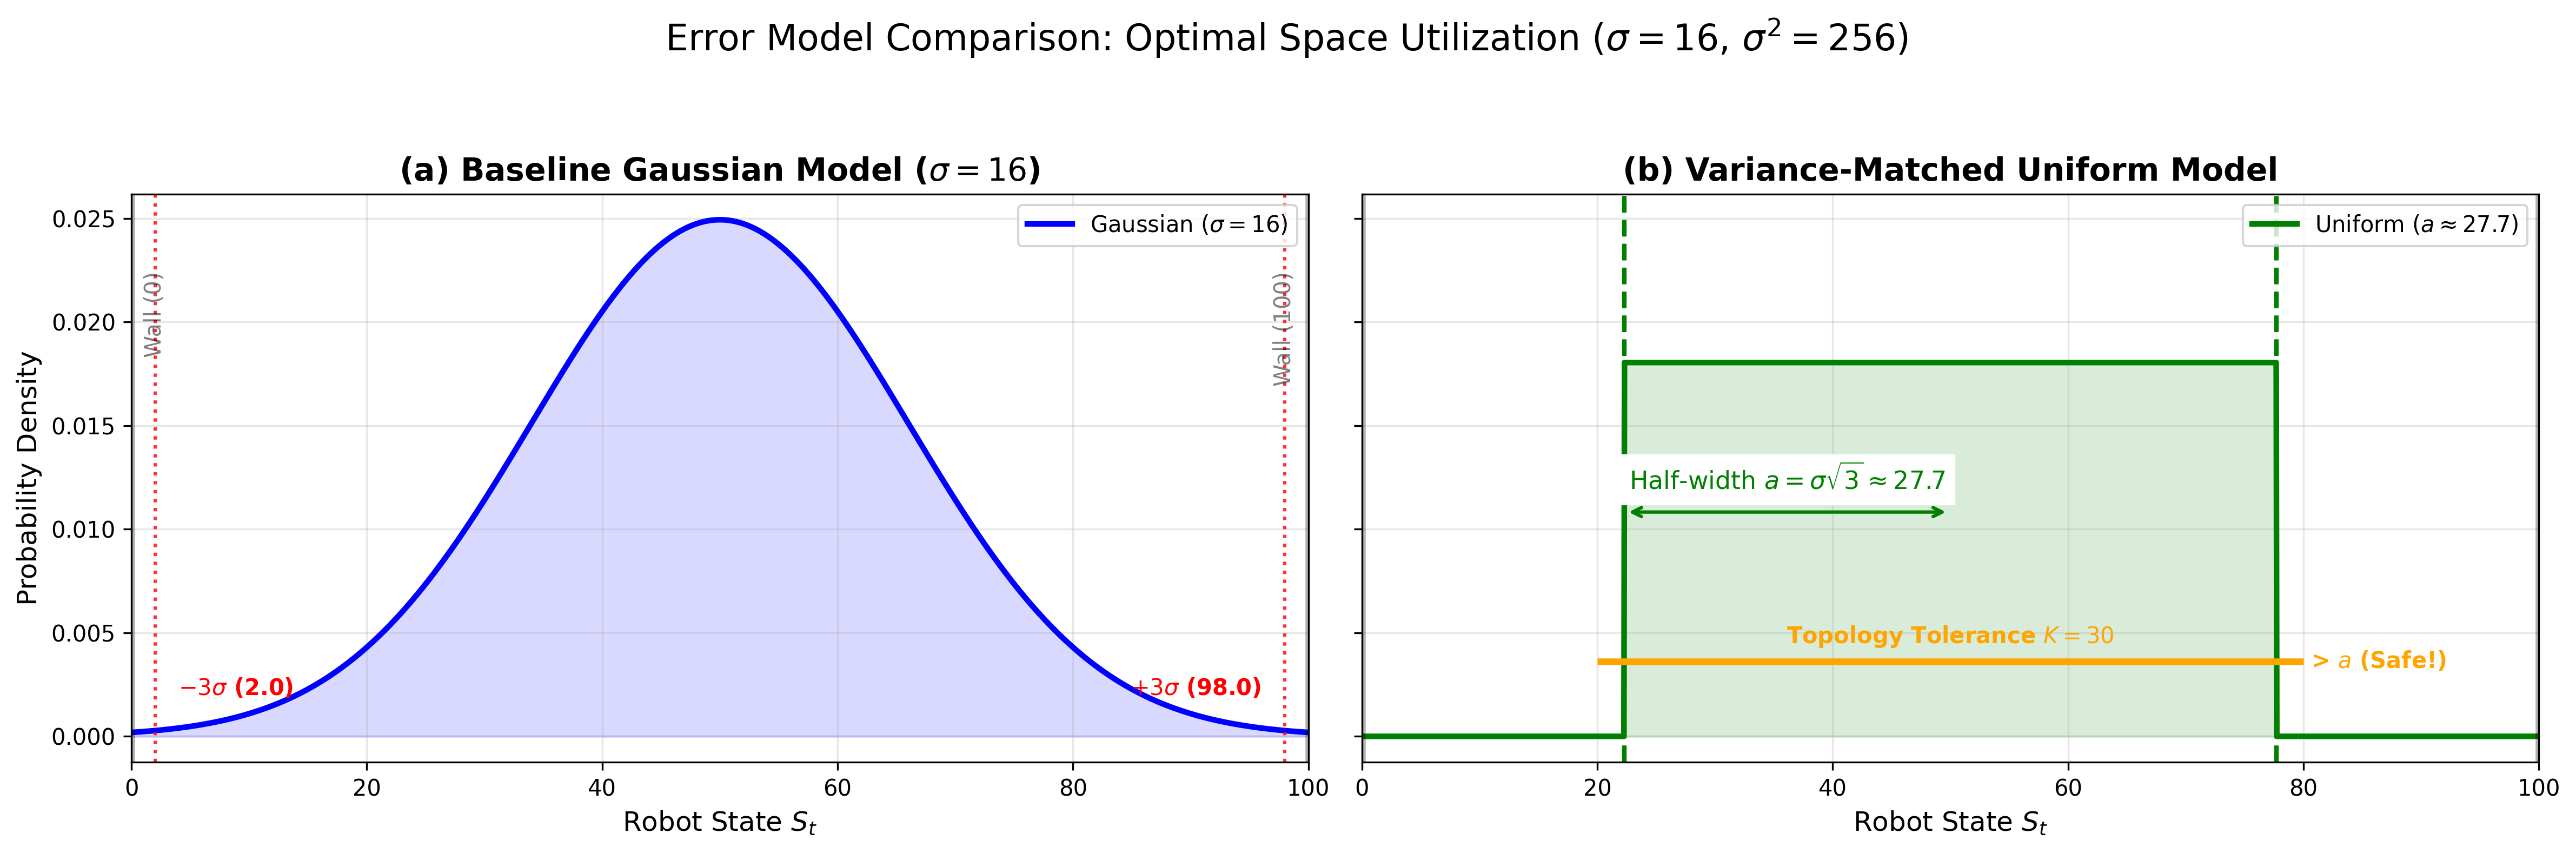
\includegraphics[width=1.0\textwidth]{figures/error_models_sigma16.png}
    \caption{Visual comparison of the variance-matched error models configured with $\sigma=16$. The Gaussian baseline (a) maximizes physical space utilization within the domain bounds $[2, 98]$, preventing truncation artifacts while maintaining high noise energy. The Uniform model (b) illustrates the safe-harbor threshold: the selected tolerance radius of 30 exceeds the noise support, guaranteeing zero tolerance-violation risk under the Uniform model, whereas the Gaussian model retains residual tail risks outside the tolerance zone.}
    \label{fig:error_models}
\end{figure}

\subsection{Computational Scalability and Latency Model}
\label{subsec:scalability_model}

A sensitivity analysis quantifies the computational scalability of the \gls{kid} decoder by sweeping the quantization resolution $\Delta$ from 1.0 down to 0.01. The total decoder latency is modeled linearly as the product of the acceptance-set cardinality $K$ and the unit verification overhead; since $K$ grows approximately as $K\propto R/\Delta$ (Equation~\eqref{eq:kid_K_from_R}), finer quantization increases computation even when $R$ is fixed.

The results of this sensitivity sweep reveal a scalability bottleneck governed by the resolution. As the quantization becomes finer, the computational cost grows hyperbolically. For large-tolerance configurations, high-precision settings drive the decoder latency well beyond typical control budgets. Relaxing the resolution to 0.1 reduces the worst-case latency to approximately 1.3 ms, balancing precision with feasibility. Consequently, this operating point is selected as the fixed resolution for subsequent experiments.

\begin{figure}[H]
    \centering
    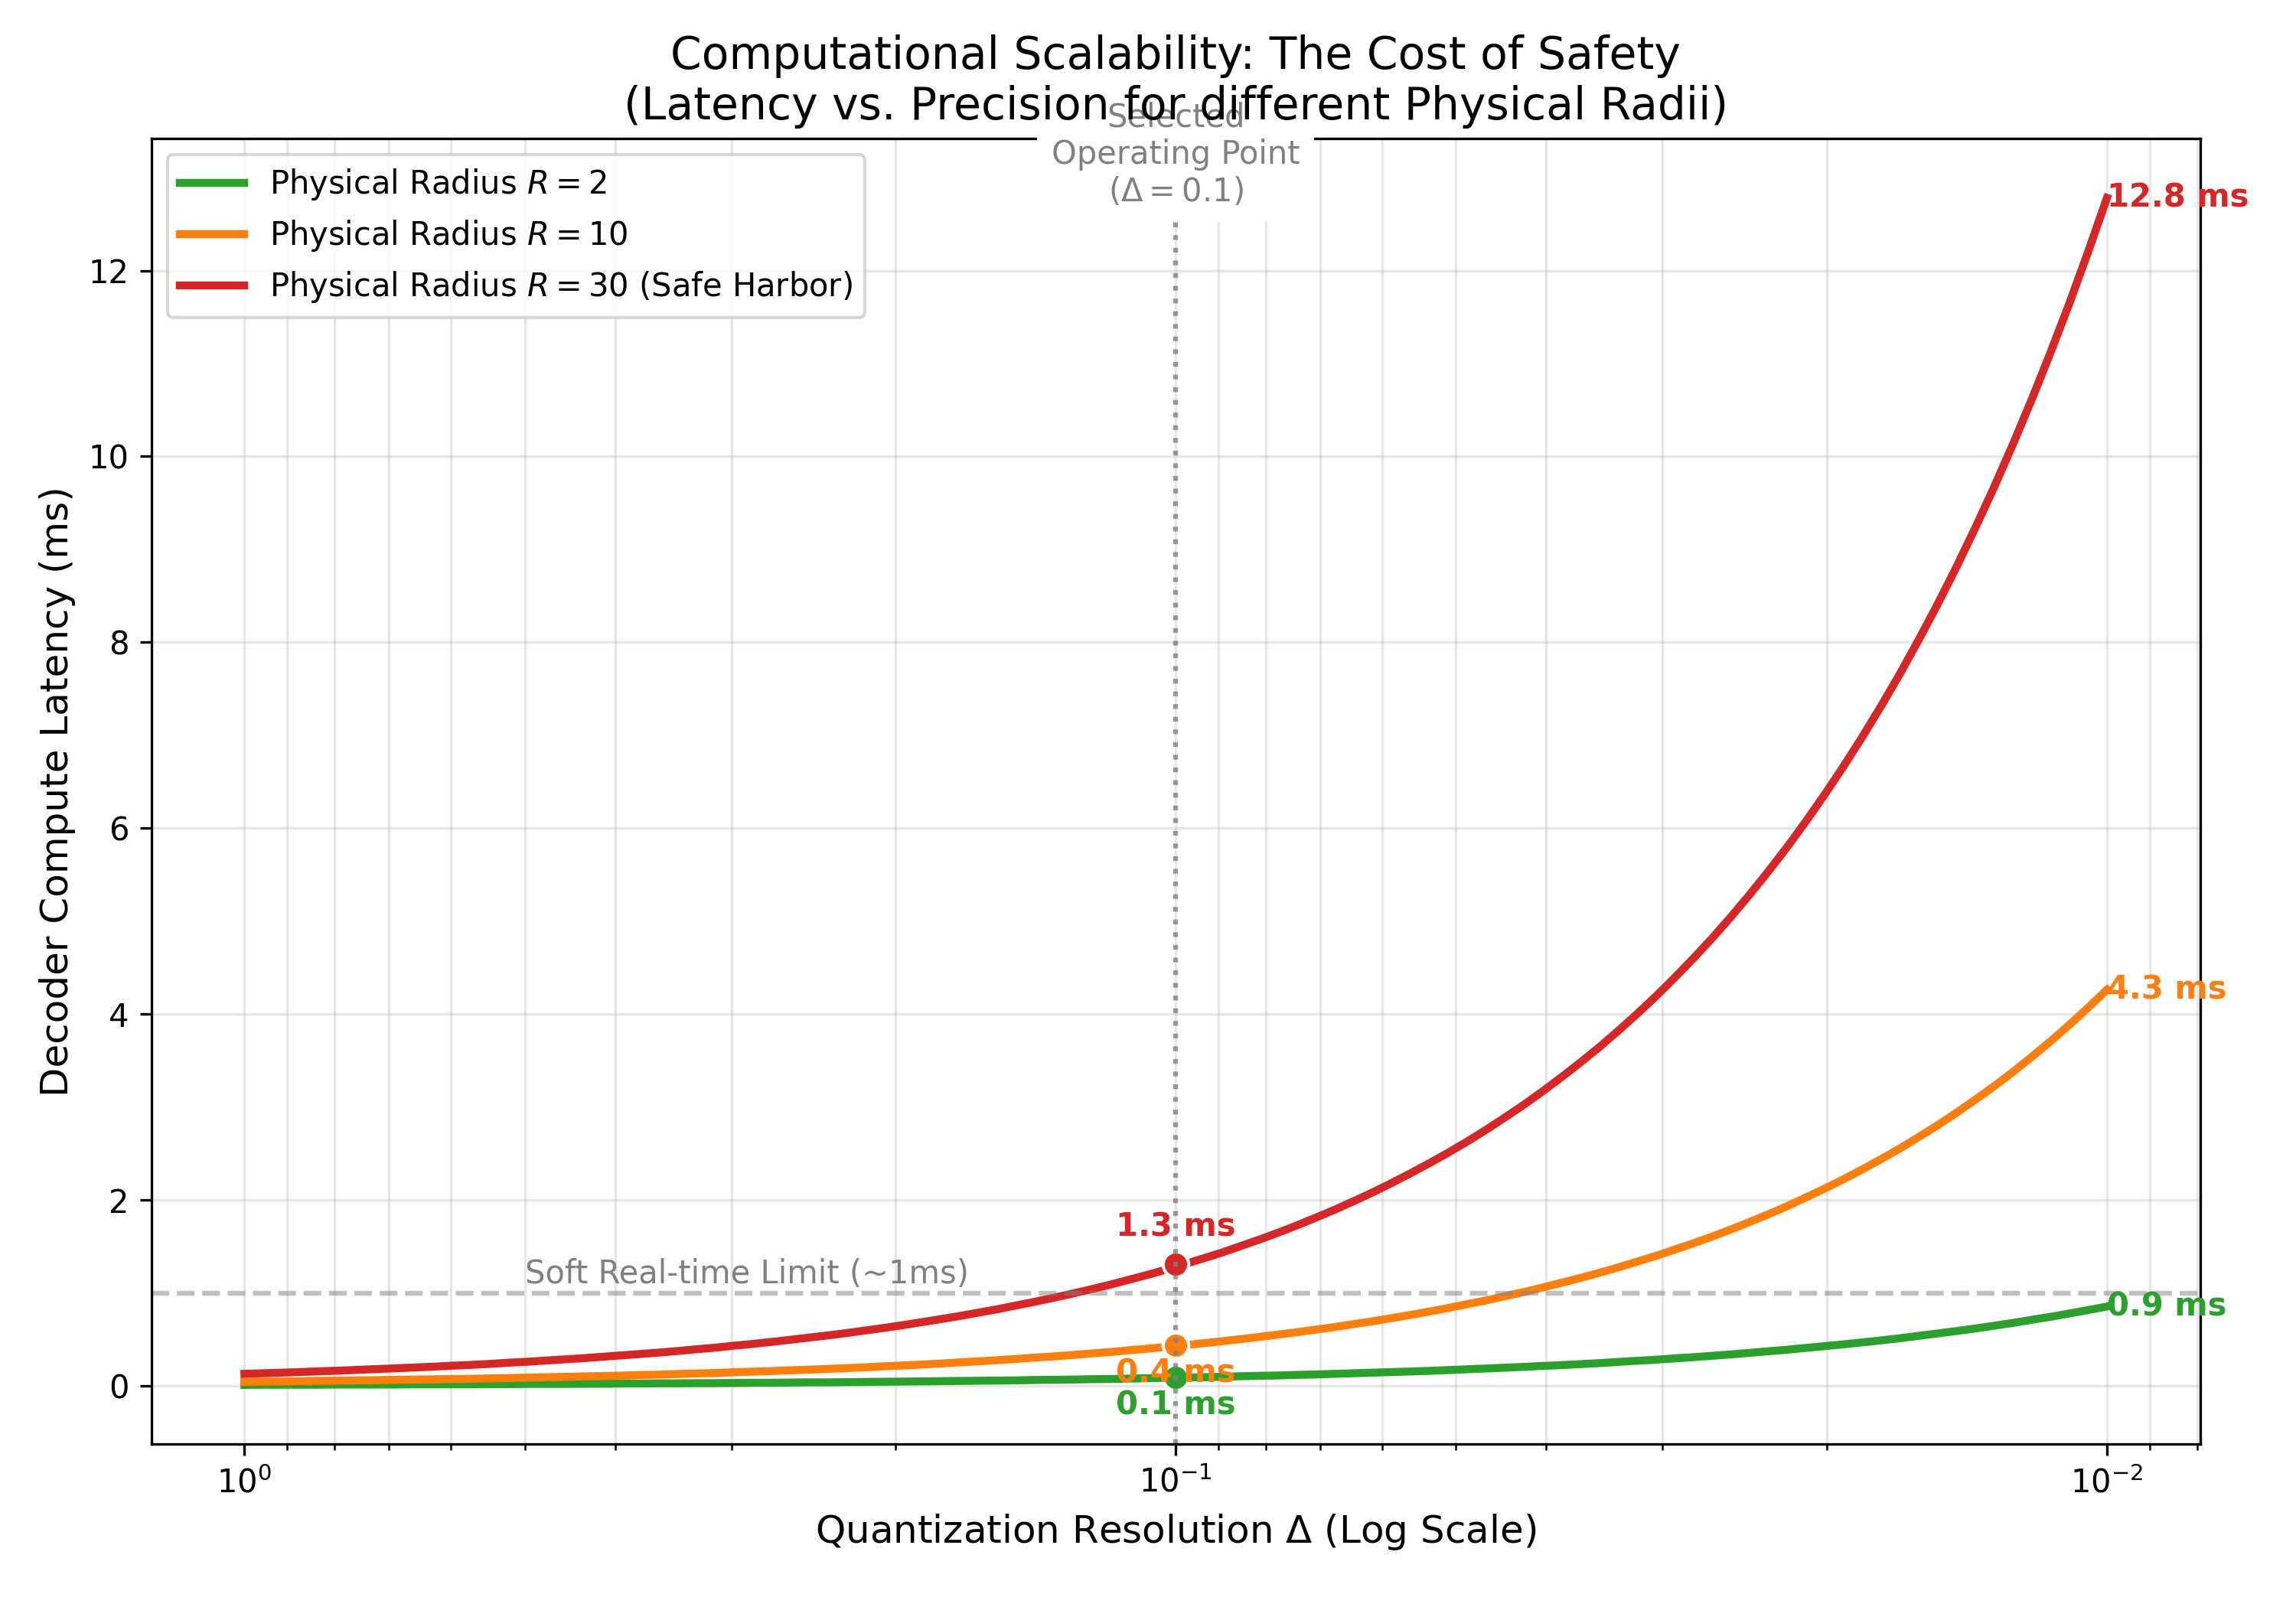
\includegraphics[width=0.72\linewidth,height=0.32\textheight,keepaspectratio]{figures/decoder_cost_multiline_annotated.png}
    \caption{Computational scalability analysis showing decoder latency as a function of quantization resolution $\Delta$. The red curve represents the safe-harbor configuration ($R=30$). At the high-precision limit ($\Delta=0.01$), latency reaches a prohibitive 12.8 ms. However, at the selected operating point ($\Delta=0.1$, indicated by the vertical dotted line), the latency drops to approximately 1.3 ms, balancing maximum physical coverage with real-time computational feasibility.}
    \label{fig:decoder_scalability}
\end{figure}

\subsection{System Configuration and Visualization}
\label{subsec:param_config}

The primary simulation assumes a payload of 4001 bits transmitted over a 1 Mbps link. The evaluation framework employs the physical tolerance radius $R$ as the primary independent variable to maintain a direct mapping to robotic safety requirements. The sweep uses $R\in\{2,5,10,20,30\}$. The largest value is motivated by the Uniform half-width derived above ($a\approx 27.71$), which provides a boundary condition where tolerance violations vanish under bounded noise.

To analyze the trade-off space, a dual visualization strategy is employed. Raw simulation results are mapped onto a grid defined by verifier length and physical tolerance to display speedup factors and risk probabilities. These points are subsequently projected onto a risk-vs-speedup scatter plot to extract the Pareto frontier.

\section{Dynamic Evaluation Framework: The Random Walk Model}
\label{sec:dynamic_evaluation}

To evaluate \gls{kid} under continuous operation, a discrete-time simulation framework is used comprising a stochastic robot agent, a bandwidth-constrained channel, and a \gls{dt} receiver. Unlike the static sweeps in Section~\ref{sec:kid_setup}, this dynamic evaluation models time-correlated accumulation of drift, allowing safety risks that only emerge over extended trajectories to be quantified.

\subsection{Dynamic Protocol Logic}
The robot's state evolution is modeled as a diffusive process, specifically a Gaussian random walk defined by $S_t = S_{t-1} + \delta_t$, where the increment follows a normal distribution with a unit step deviation. This standardized diffusion ensures the variance of the uncorrected state grows linearly with time, providing a reproducible challenge for the synchronization protocol.

The \gls{kid} protocol operates as a guardrail mechanism on this state evolution. At each time tick, the absolute deviation between the true state and the \gls{dt} estimate is evaluated. If the deviation remains within the tolerance radius ($|e|\le R$), the protocol remains silent; if $|e|>R$, a verification event is triggered.

For long-horizon simulation, the encoder backend is abstracted as a probabilistic verification model grounded in the Chapter~2 reliability law (Equation~\eqref{eq:pmiss_law}). Specifically, the verification outcome at a check event is implemented as a Bernoulli trial with miss probability $p_{miss}\approx K/2^{n_{ver}}$, where $K=|\mathcal{A}_R|$ is induced by $(R,\Delta)$ (Equation~\eqref{eq:kid_K_from_R}). This abstraction preserves the theoretically derived dependence on $(K,n_{ver})$ while decoupling the experiment logic from implementation-specific hashing costs.

\subsection{Experimental Strategy}
The evaluation strategy consists of two complementary phases. First, a qualitative stress test is used to induce observable failure modes. By intentionally reducing $n_{ver}$, the collision probability increases, which amplifies otherwise rare long-tail events and makes sustained boundary breaches observable within a manageable simulation window.

Second, a quantitative parameter sweep systematically varies the tolerance radius and verifier length while fixing the drift dynamics. This grid search decouples the masking effect of physical tolerance from the collision risk of the verification step, providing the statistical basis for the trade-off analysis.

\subsection{Metrics for Dynamic Safety}
To quantify the trade-off between efficiency and risk, three primary metrics are defined. The Successive Recovery Interval (\gls{sri}) measures the number of ticks between two consecutive recovery-triggered check events (i.e., transmission attempts triggered by $|E_t|>R$). In the simulator, this quantity is equivalent to the inter-check interval (\gls{ift}); a larger \gls{sri} indicates higher masking efficiency and reduced channel contention.

Safety is assessed via two complementary metrics. The Breach Duration counts the number of consecutive ticks during which the system remains in an unsafe state due to hash collisions, measuring the temporal persistence of safety violations. Finally, the Maximum Drift metric records the peak absolute error reached during a simulation run. Unlike Breach Duration, this quantifies the worst-case physical magnitude of the error, serving as a proxy for potential physical damage in control scenarios.


\chapter{Results and Evaluation}
\label{ch:results}
\label{sec:results_and_evaluation}

\section{Empirical Parameter Verification}
To instantiate the theoretical models derived in Chapter~\ref{ch:design_methodology}, we first characterize the system parameters experimentally. This includes measuring the computational overhead ($t_{ver}$) and calculating the theoretical collision probabilities ($p_{miss}$).

\subsection{Encoding Latency ($t_{ver}$)}
The computational overhead of the encoding step, $t_{ver}$, was measured empirically by running 100{,}000 \texttt{send} operations for each system configuration. In addition to the sample mean, we estimate a \textbf{95\% confidence interval (CI)} for the mean using a batch timing method (100 timing batches, each covering an equal share of operations).

\textbf{Interpretation of Table~\ref{tab:tver_results_bits}:}
The table reports the \emph{sample mean} $\bar{t}_{ver}$ in microseconds. The CI quantifies measurement uncertainty due to runtime noise (OS scheduling, cache effects, Python overhead). In our measurements, the 95\% CI half-widths are below \textbf{1\,$\mu s$} for all configurations. Therefore, the reported means are sufficiently stable for the latency-model comparisons in this chapter.

Note that the \textbf{mean} values can shift slightly across runs and machines (Python runtime, CPU frequency scaling, background load). For reproducibility and consistency with the figures in this chapter, we keep the table mean values aligned with the parameter set used for the plotted latency evaluation, and we report representative 95\% CI half-widths to quantify the measurement uncertainty.

\begin{table}[!htbp]  % Prefer LaTeX float placement (float package not required)
    \centering
    \caption{Measured Verification Time $t_{ver}$ (mean $\pm$ 95\% CI half-width, with relative half-width)}
    \label{tab:tver_results_bits}
    \begin{tabular}{lrr}
        \toprule
        & \multicolumn{2}{c}{$n_{ver}$ (bits)} \\
        \cmidrule(lr){2-3}
        System ($n_{data}$) & 4 & 16 \\
        \midrule
        \textbf{SHA-256} & & \\
        96 bits & $2.13\pm0.04\,(1.9\%)$ & $2.24\pm0.01\,(0.4\%)$ \\
        4001 bits & $14.65\pm0.31\,(2.1\%)$ & $15.41\pm0.09\,(0.6\%)$ \\
        \midrule
        \textbf{RS-ID} & & \\
        96 bits & $14.55\pm0.39\,(2.7\%)$ & $3.79\pm0.02\,(0.5\%)$ \\
        4001 bits & $51.78\pm0.94\,(1.8\%)$ & $38.57\pm0.36\,(0.9\%)$ \\
        \bottomrule
    \end{tabular}
\end{table}

\textbf{Analysis of $t_{ver}$ Results:}
The measurement results in Table~\ref{tab:tver_results_bits} reveal distinct performance characteristics between the algebraic (RS-ID) and cryptographic (SHA-256) approaches:

\begin{enumerate}
    \item \textbf{Stability of SHA-256:} Consistent with the theoretical discussion in Section~\ref{sec:reliability_analysis}, the computation time of SHA-256 is largely insensitive to the output verifier length. For the short payload ($n_{data}=96$ bits), the latency remains nearly constant (\textasciitilde 2.2~$\mu s$) when truncating to either $n_{ver}=4$ or $n_{ver}=16$ bits. When increasing the payload to $n_{data}=4001$ bits, the latency rises to \textasciitilde 15~$\mu s$, which is expected due to the block-based processing of SHA.
    
    \item \textbf{The Chunking Effect in RS-ID:} A counter-intuitive phenomenon is observed for RS-ID: for the small payload ($n_{data}=96$ bits), increasing the verifier length from $n_{ver}=4$ to $n_{ver}=16$ bits \textit{reduces} the measured latency substantially (from 14.55~$\mu s$ to 3.79~$\mu s$).
    This can be explained by the polynomial construction mechanism. RS-ID represents the input as $k$ coefficients, where $k=\lceil n_{data}/n_{ver} \rceil$. With $n_{ver}=4$, the data is sliced into 24 chunks, requiring more iterations of field operations. With $n_{ver}=16$, the chunk count drops to 6. For small datasets, the reduction in loop iterations outweighs the increased per-operation cost of arithmetic in a larger field.
\end{enumerate}

\subsection{Theoretical Collision Probability ($p_{miss}$)}
Based on the bounds derived in Chapter~\ref{ch:design_methodology} (Equations~\eqref{eq:sha_bound} and~\eqref{eq:rsid_bound}), we compute the theoretical collision probability $p_{miss}$ for the parameter grid used in the latency model. Note that for RS-ID, if the polynomial degree exceeds the field size, the bound is capped at 1.0.

\begin{table}[!htbp] % Prefer LaTeX float placement (float package not required)
    \centering
    \caption{Theoretical Collision Probability ($p_{miss}$) for Bit-Based Parameters}
    \label{tab:pmiss_results_bits}
    \begin{tabular}{lrr}
        \toprule
        & \multicolumn{2}{c}{$n_{ver}$ (bits)} \\
        \cmidrule(lr){2-3}
        System ($n_{data}$) & 4 & 16 \\
        \midrule
        \textbf{SHA-256 (any $n_{data}$)} & $6.25\times 10^{-2}$ & $1.53\times 10^{-5}$ \\
        \midrule
        \textbf{RS-ID} & & \\
        96 bits & $1.00$ & $9.16\times 10^{-5}$ \\
        4001 bits & $1.00$ & $3.83\times 10^{-3}$ \\
        \bottomrule
    \end{tabular}
\end{table}

\section{End-to-End Latency Evaluation}
Using the hybrid latency model and the calibrated parameters from Section 5.1, we analyze the system performance across varying network conditions and prediction qualities.

\subsection{Sensitivity to Channel Bandwidth}
We first evaluate the expected latency as a function of channel bandwidth ($B$). Figures~\ref{fig:latency_vs_bandwidth_96bits} and~\ref{fig:latency_vs_bandwidth_4001bits} compare the Traditional approach against the ID-based schemes.

\begin{figure}[!htbp]
    \centering
    \begin{minipage}[t]{0.49\textwidth}
        \centering
        
\includegraphics[width=\linewidth]{figures/plots/latency_empirical_bandwidth_96bits.png}
        \captionof{figure}{Expected latency vs. bandwidth for $n_{data}=96$ bits ($p_{desync}=0.1$).}
        \label{fig:latency_vs_bandwidth_96bits}
    \end{minipage}\hfill
    \begin{minipage}[t]{0.49\textwidth}
        \centering
        
\includegraphics[width=\linewidth]{figures/plots/latency_empirical_bandwidth_4001bits.png}
        \captionof{figure}{Expected latency vs. bandwidth for $n_{data}=4001$ bits ($p_{desync}=0.1$).}
        \label{fig:latency_vs_bandwidth_4001bits}
    \end{minipage}
\end{figure}

\textbf{Discussion (Bandwidth Trade-off):}
The results illustrate the dominance of the Identification scheme in bandwidth-constrained environments. 
\begin{itemize}
    \item \textbf{Low Bandwidth Regime ($B < 1$ Mbps):} The transmission time of raw data dominates the Traditional latency. The ID scheme offers an order-of-magnitude reduction by transmitting only the compact verifier.
    \item \textbf{High Bandwidth Regime ($B > 10$ Mbps):} As transmission becomes instantaneous, the latency floor is determined by the computational overhead $t_{ver}$. Consequently, the Traditional scheme (which has zero encoding overhead) eventually outperforms the ID schemes, creating a clear "Cross-over Point."
\end{itemize}

\subsection{Sensitivity to Prediction Quality}
Next, we examine the impact of the Digital Twin's prediction accuracy ($p_{desync}$) at a fixed bandwidth ($B=5$ Mbps).

\begin{figure}[!htbp]
    \centering
    \begin{minipage}[t]{0.49\textwidth}
        \centering
        
\includegraphics[width=\linewidth]{figures/plots/latency_vs_desync_96bits.png}
        \captionof{figure}{Expected latency vs. $p_{desync}$ for $n_{data}=96$ bits ($B=5$ Mbps).}
        \label{fig:latency_vs_desync_96bits}
    \end{minipage}\hfill
    \begin{minipage}[t]{0.49\textwidth}
        \centering
        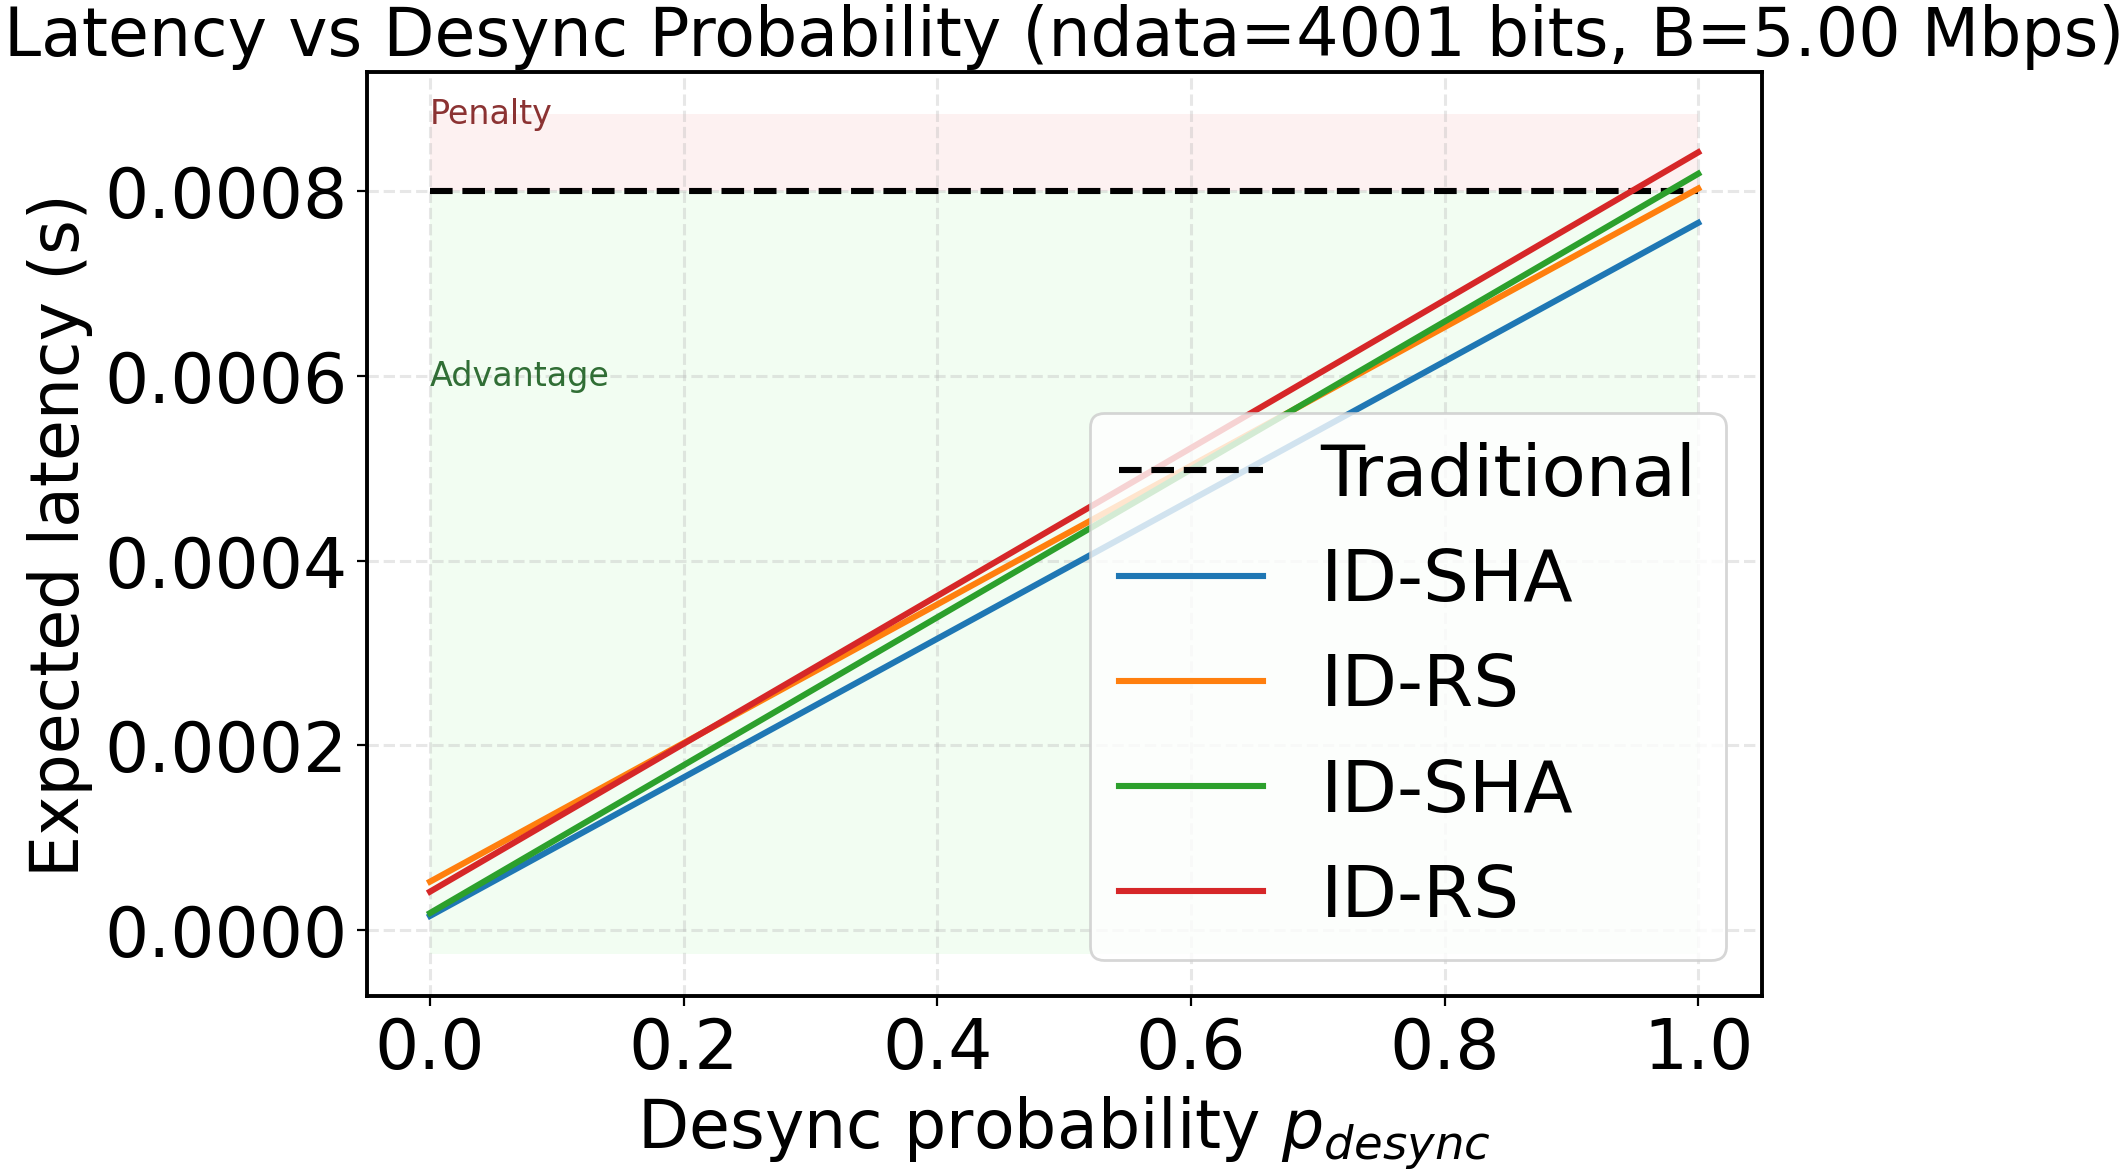
\includegraphics[width=\linewidth]{figures/plots/latency_vs_desync_4001bits.png}
        \captionof{figure}{Expected latency vs. $p_{desync}$ for $n_{data}=4001$ bits ($B=5$ Mbps).}
        \label{fig:latency_vs_desync_4001bits}
    \end{minipage}
\end{figure}

\textbf{Discussion (Prediction Quality):}
\begin{itemize}
    \item \textbf{Break-even Analysis:} For the short payload (Fig.~\ref{fig:latency_vs_desync_96bits}), the ID-SHA curves intersect the Traditional line at approximately $p_{desync} \approx 0.8$. This implies that ID is beneficial as long as the Digital Twin's prediction accuracy exceeds 20\%. For the large payload (Fig.~\ref{fig:latency_vs_desync_4001bits}), the transmission penalty is so high that ID-SHA remains superior across nearly the entire range of $p_{desync}$.
    
    \item \textbf{Anomaly Analysis (RS-ID $n_{ver}=4$):} 
    A notable anomaly appears in the RS-ID results for $n_{ver}=4$ bits (orange line in Fig.~\ref{fig:latency_vs_desync_96bits}), which appears flat and low. This is a \textbf{theoretical artifact} caused by the saturation of collision probability ($p_{miss}=1.0$, see Table~\ref{tab:pmiss_results_bits}). Mathematically, this sets the fallback penalty term to zero. In reality, this represents a catastrophic failure where desynchronization is never detected. Therefore, this configuration is invalid for safety-critical systems despite its apparent low latency.
\end{itemize}

\section{K-ID Safety--Latency Trade-off}
\label{sec:kid_results}
This section evaluates the tolerance-based K-ID model introduced in Section~\ref{sec:kid_model} and implemented as described in Section~\ref{sec:kid_setup}. The experiment sweeps $n_{ver}\in\{4,8,12,16\}$ and $K\in\{2,5,10,20\}$ for a 96-bit payload at $B=1$ Mbps.

\subsection{Sweep Results}
Figure~\ref{fig:kid_sweep_overview} summarizes the main metrics. The miss rate is plotted as the conditional safety risk $\Pr[\mathrm{accept}\mid\mathrm{unsafe}]$, i.e., the probability that an unsafe state is incorrectly accepted due to a verifier collision with the acceptable set.

\begin{figure}[!htbp]
    \centering
    \begin{subfigure}[t]{0.49\textwidth}
        \centering
        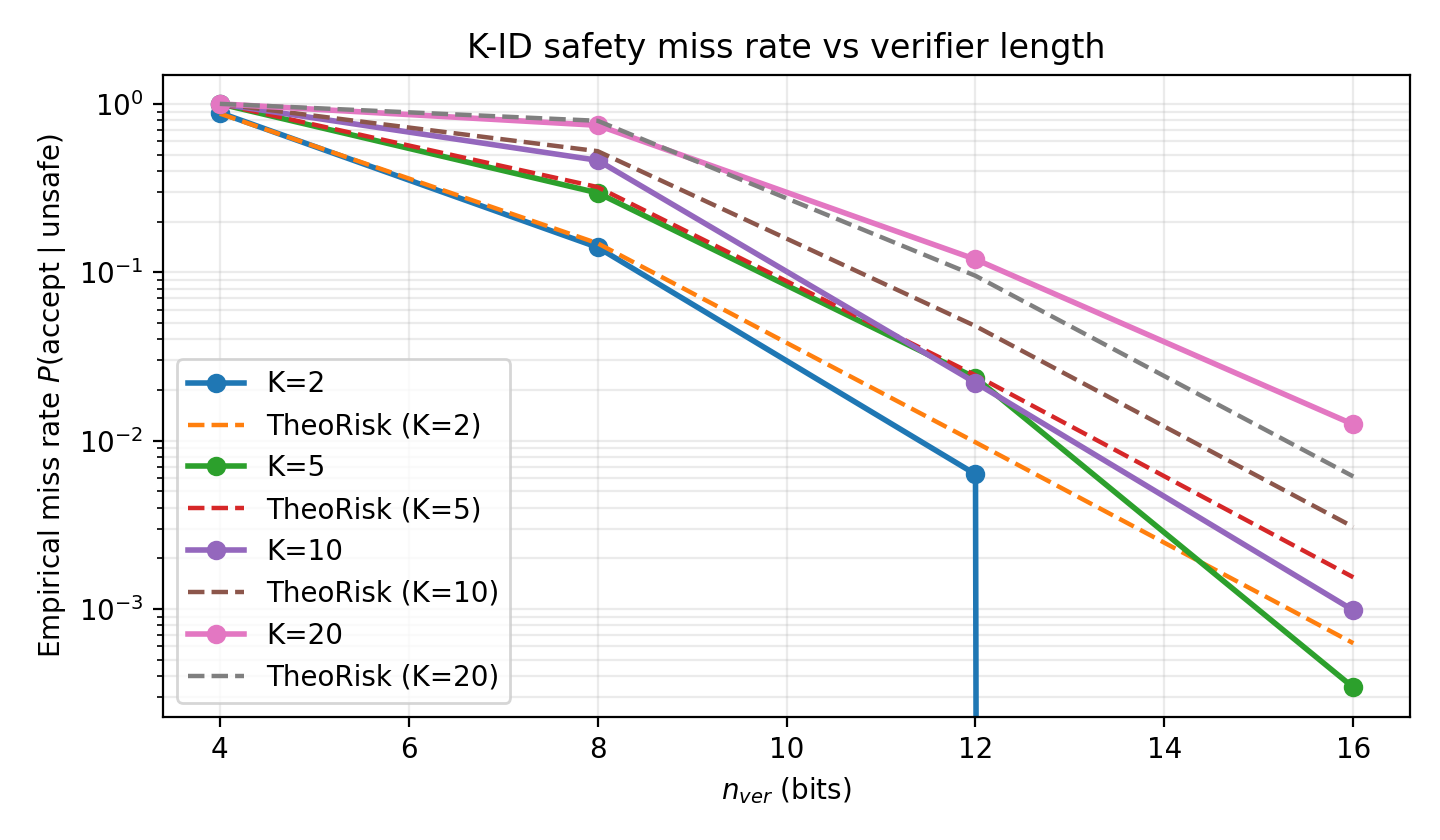
\includegraphics[width=\linewidth]{figures/plots/kid_sweep_miss_rate.png}
        \caption{Conditional miss rate $\Pr[\mathrm{accept}\mid\mathrm{unsafe}]$.}
        \label{fig:kid_miss_rate}
    \end{subfigure}\hfill
    \begin{subfigure}[t]{0.49\textwidth}
        \centering
        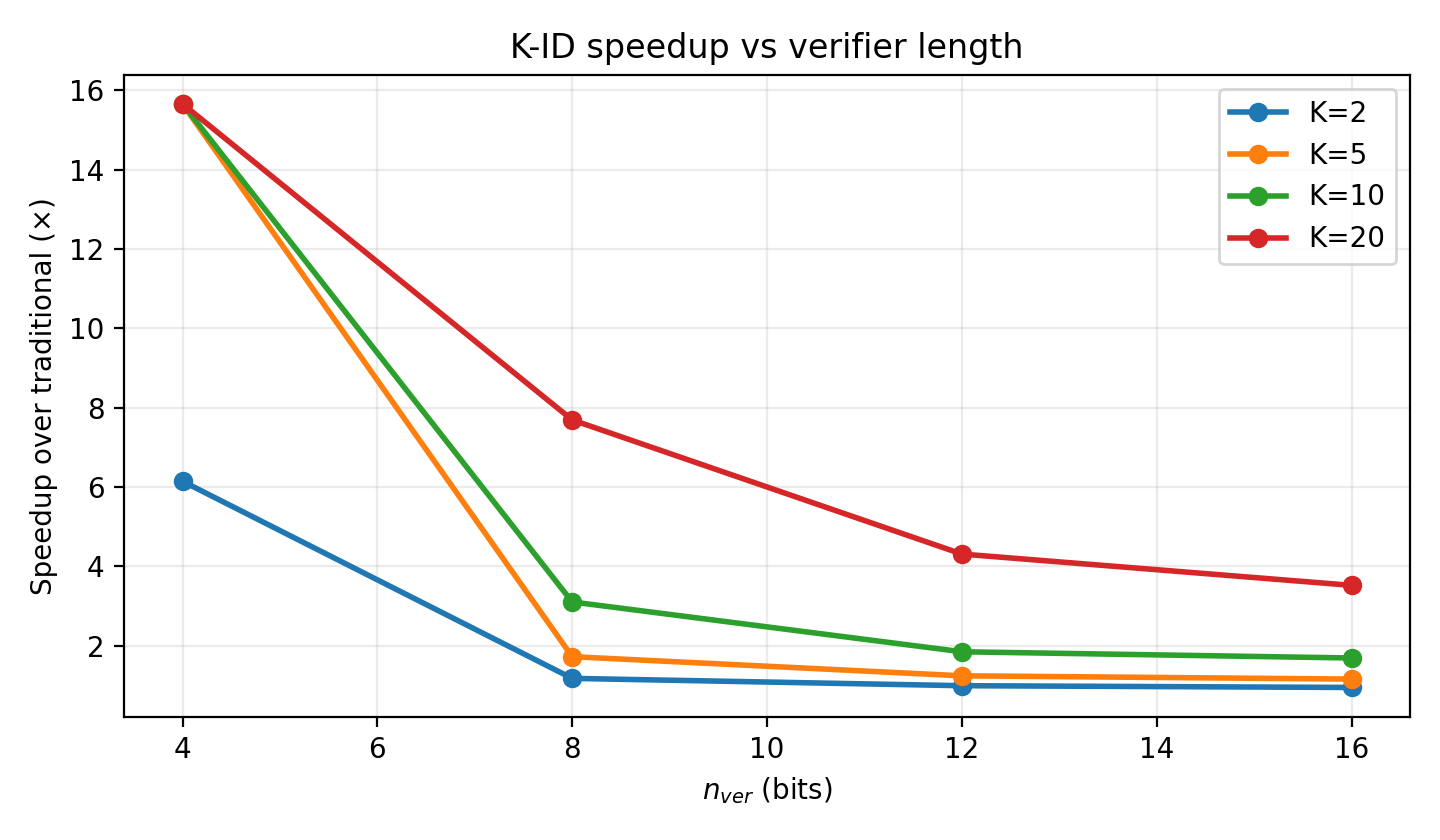
\includegraphics[width=\linewidth]{figures/plots/kid_sweep_speedup.png}
        \caption{Speedup over traditional transmission.}
        \label{fig:kid_speedup}
    \end{subfigure}

    \vspace{0.6em}

    \begin{subfigure}[t]{0.49\textwidth}
        \centering
        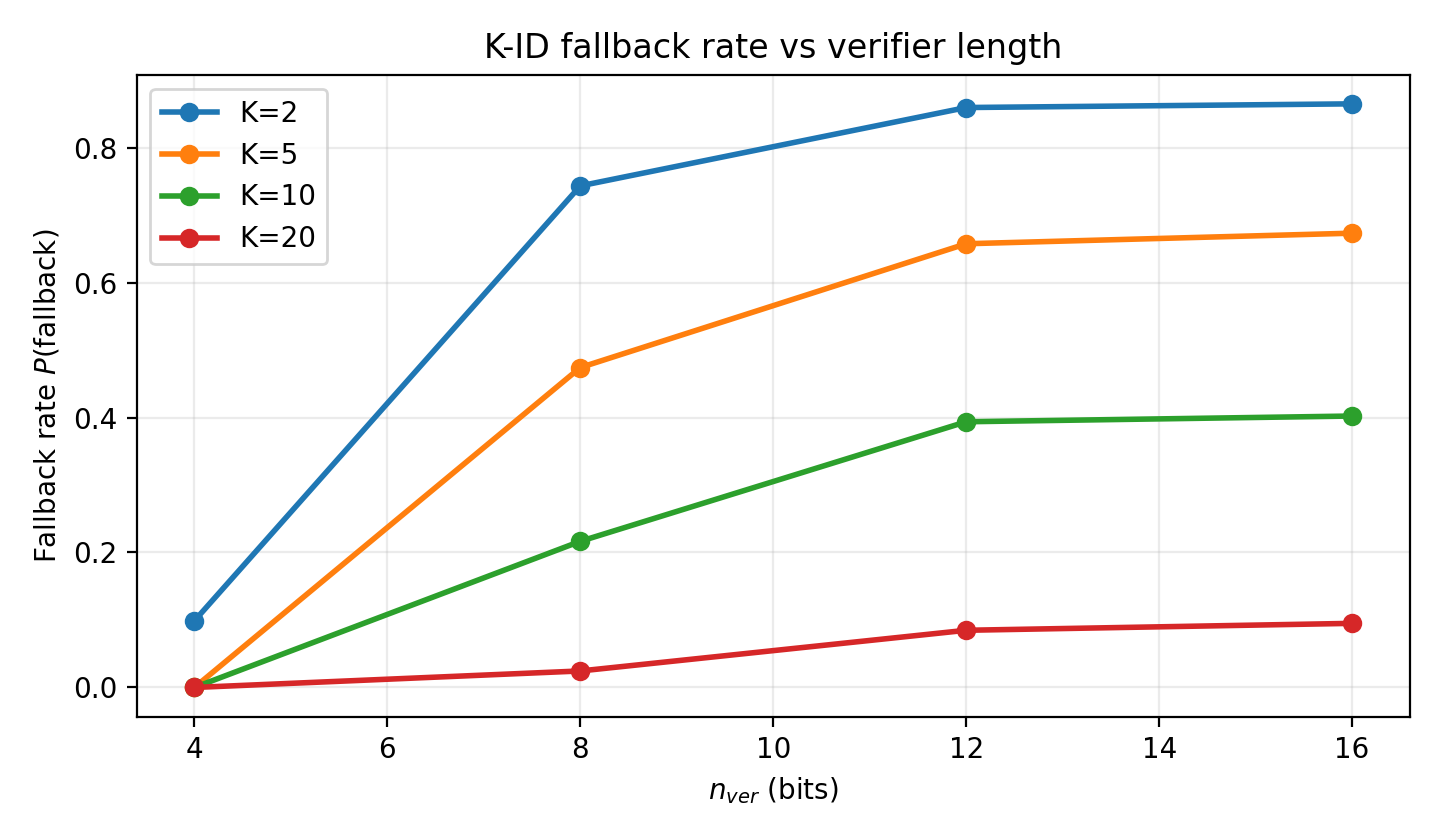
\includegraphics[width=\linewidth]{figures/plots/kid_sweep_fallback_rate.png}
        \caption{Fallback probability $\Pr[\mathrm{fallback}]$.}
        \label{fig:kid_fallback_rate}
    \end{subfigure}\hfill
    \begin{subfigure}[t]{0.49\textwidth}
        \centering
        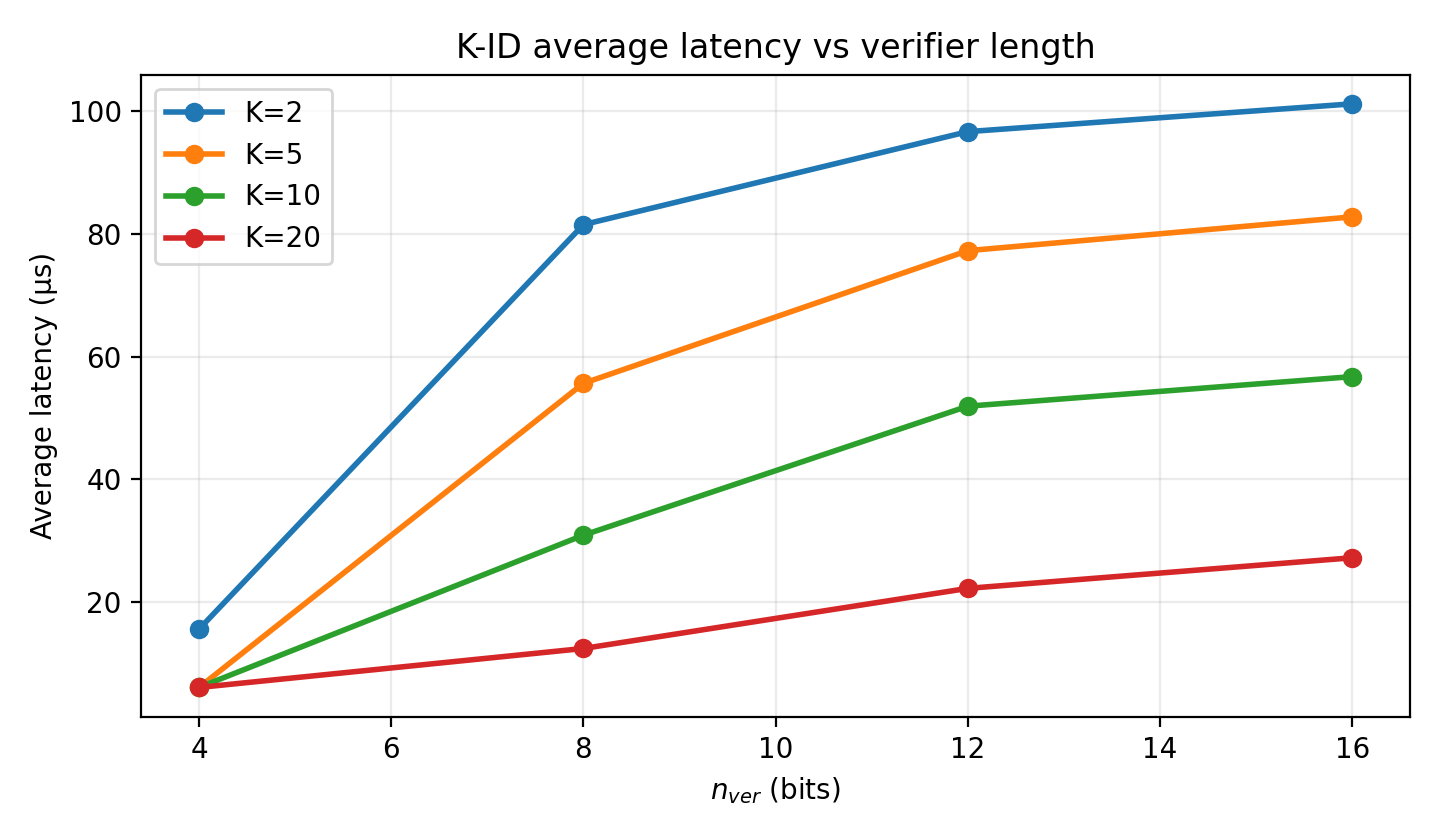
\includegraphics[width=\linewidth]{figures/plots/kid_sweep_latency.png}
        \caption{Expected latency under Equation~\eqref{eq:kid_latency}.}
        \label{fig:kid_latency}
    \end{subfigure}

    \caption{K-ID parameter sweep results for $n_{data}=96$ bits at $B=1$ Mbps.}
    \label{fig:kid_sweep_overview}
\end{figure}

\textbf{Analysis (Effect of $n_{ver}$):}
Increasing $n_{ver}$ reduces the conditional miss rate approximately exponentially, consistent with the Random Oracle scaling in Equation~\eqref{eq:kid_sha_bound}. However, a larger $n_{ver}$ also increases the mandatory verifier transmission term $n_{ver}/B$ and, more importantly, reduces the chance of ``accidental acceptance'' when unsafe, which increases detection and therefore increases fallback frequency. As a result, higher $n_{ver}$ improves safety but can reduce speedup (and increase latency) depending on how often the system enters unsafe states.

\textbf{Analysis (Effect of $K$):}
Increasing $K$ enlarges the acceptable set. This has two opposing effects that are visible in Figure~\ref{fig:kid_sweep_overview}:
\begin{itemize}
    \item The conditional miss rate $\Pr[\mathrm{accept}\mid\mathrm{unsafe}]$ increases with $K$, because more acceptable states mean more opportunities for a hash collision with an unsafe verifier.
    \item The fallback rate and latency decrease with $K$ because the system is unsafe less often (fewer ticks lie outside the tolerance interval), so the expensive full-payload fallback is triggered less frequently.
\end{itemize}
This demonstrates the fundamental K-ID trade-off: a larger tolerance improves performance and reduces fallback, but raises the conditional risk of accepting an unsafe state.

\subsection{Pareto Frontier Interpretation}
To make the trade-off explicit, Figure~\ref{fig:kid_pareto} plots speedup against the \emph{conditional} miss rate $P(\mathrm{accept}\mid\mathrm{unsafe})$ and highlights the non-dominated (Pareto-optimal) configurations.

\begin{figure}[!htbp]
    \centering
    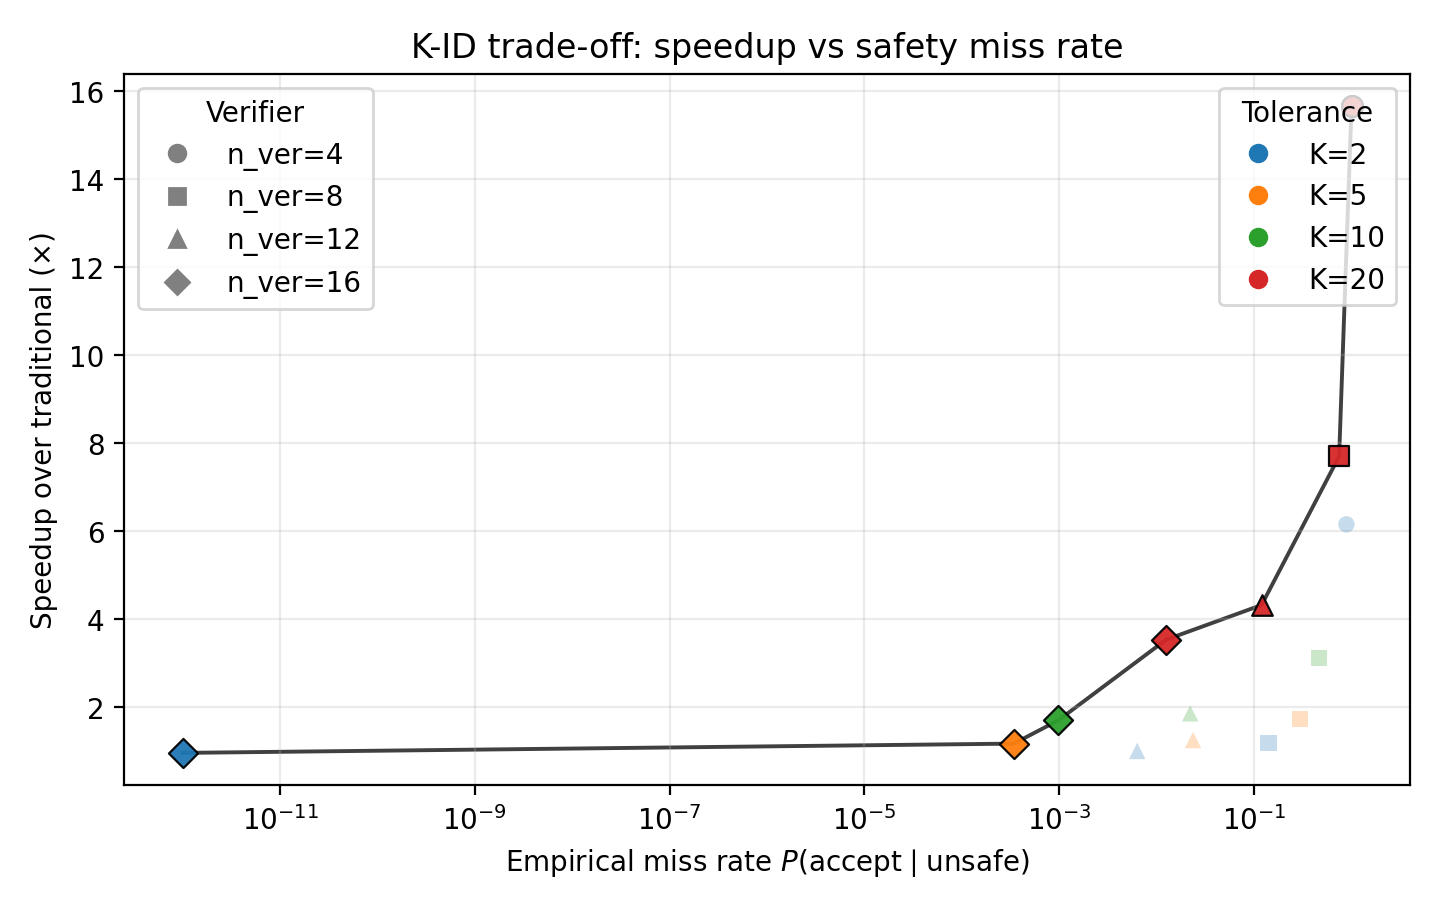
\includegraphics[width=0.72\textwidth]{figures/plots/kid_sweep_pareto.png}
    \caption{Pareto view of the K-ID trade-off: speedup vs. conditional miss rate $P(\mathrm{accept}\mid\mathrm{unsafe})$.}
    \label{fig:kid_pareto}
\end{figure}

\textbf{Overall Risk vs. Conditional Miss Rate:}
The x-axis in Figure~\ref{fig:kid_pareto} is a \emph{conditional} safety metric: it describes how likely an unsafe state is accepted \emph{given that} the system is already unsafe. To assess end-to-end operational risk, it is often more informative to consider the \emph{overall} probability of an unsafe acceptance per tick,
\begin{equation}
    P(\mathrm{unsafe}\cap\mathrm{accept}) = P(\mathrm{unsafe})\cdot P(\mathrm{accept}\mid\mathrm{unsafe}).
\end{equation}
This overall risk accounts for how frequently unsafe states occur (which depends strongly on $K$ and the prediction error distribution). Figure~\ref{fig:kid_pareto_overall} therefore replots the trade-off using $P(\mathrm{unsafe}\cap\mathrm{accept})$ on the x-axis.

\begin{figure}[!htbp]
    \centering
    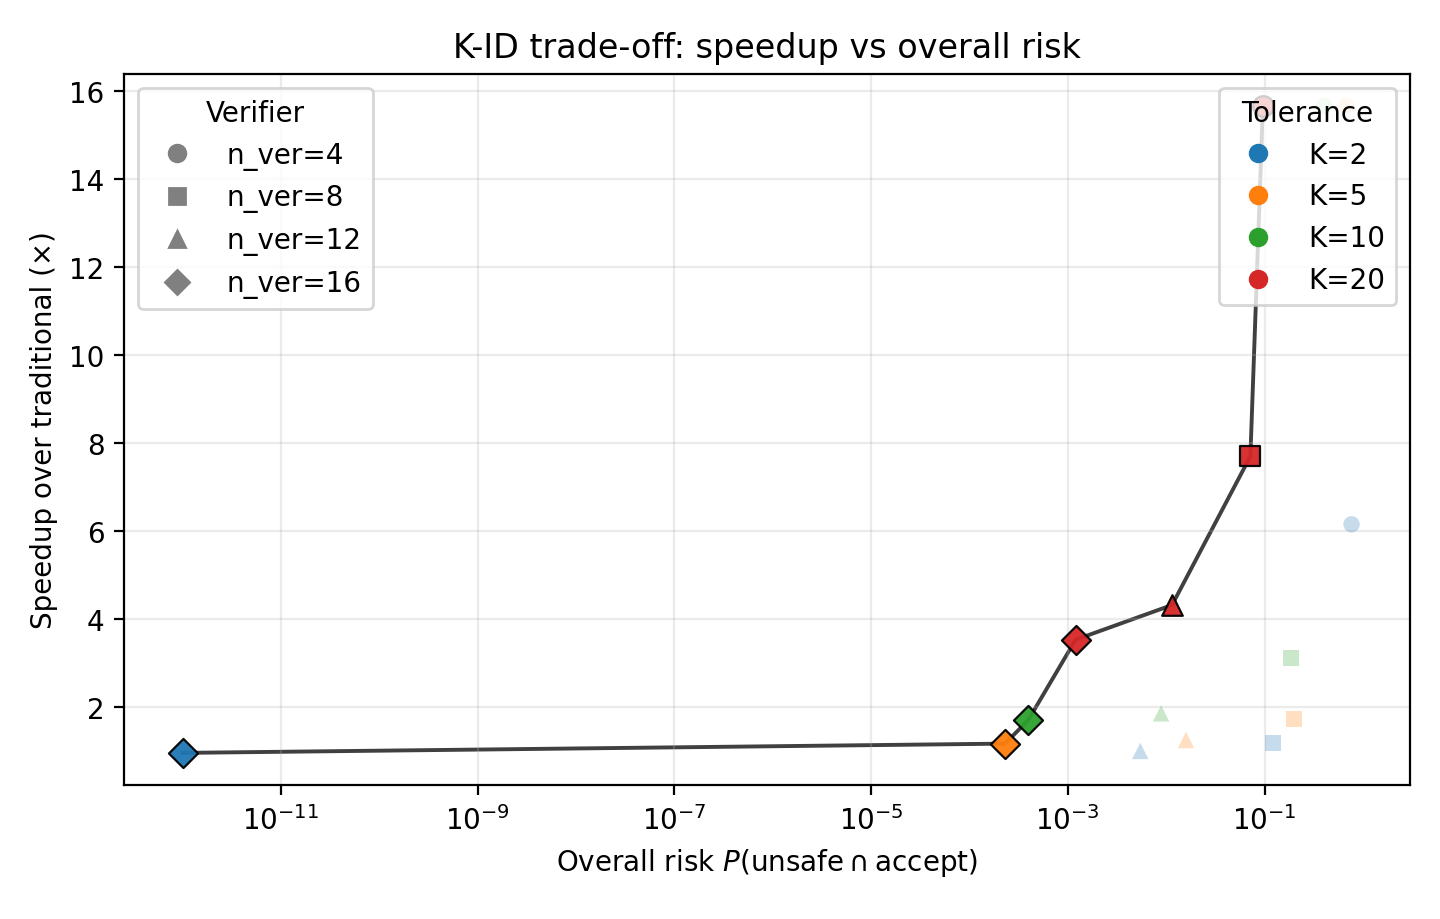
\includegraphics[width=0.72\textwidth]{figures/plots/kid_sweep_pareto_overall_risk.png}
    \caption{Pareto view using overall risk $P(\mathrm{unsafe}\cap\mathrm{accept})$: speedup vs. total unsafe-accept probability per tick.}
    \label{fig:kid_pareto_overall}
\end{figure}

\textbf{Discussion:}
The solid curve in Figure~\ref{fig:kid_pareto} connects the Pareto-optimal configurations (the \emph{frontier}). These points represent operating choices where improving safety (moving left, lower conditional miss rate) necessarily requires sacrificing speedup (moving down), and vice versa. Points in the lower-right region are \emph{dominated} (simultaneously slower and less safe) and can be discarded.

In deployment, the choice of $(K,n_{ver})$ should be driven by an application-level safety budget on $p_{miss,K}$ (or an overall risk measure that also weights the unsafe frequency) together with a latency target. The sweep provides a practical menu of operating points to select from based on these constraints.

\subsection{RS-ID Comparison and Uniform Error Model}
The baseline K-ID sweep above uses a truncated SHA-256 verifier and a Gaussian prediction error. To compare against the algebraic verifier family, we rerun the sweep with an \textbf{RS-ID} verifier (single-tag, tag position 2) and replace the error model with a \textbf{uniform} distribution centered at the mean. The uniform half-width is chosen to match the variance of the Gaussian case ($a=\sqrt{3}\,\sigma$).

Figure~\ref{fig:kid_uniform_compare} shows the resulting metrics side-by-side for \texttt{sha256\_trunc} and \texttt{rsid}. The overall trends remain consistent with the K-ID model: increasing $n_{ver}$ reduces collision-driven acceptance, while increasing $K$ reduces fallback frequency (by making unsafe states rarer), at the cost of enlarging the acceptable set.

\begin{figure}[!htbp]
    \centering
    \begin{subfigure}[t]{0.49\textwidth}
        \centering
        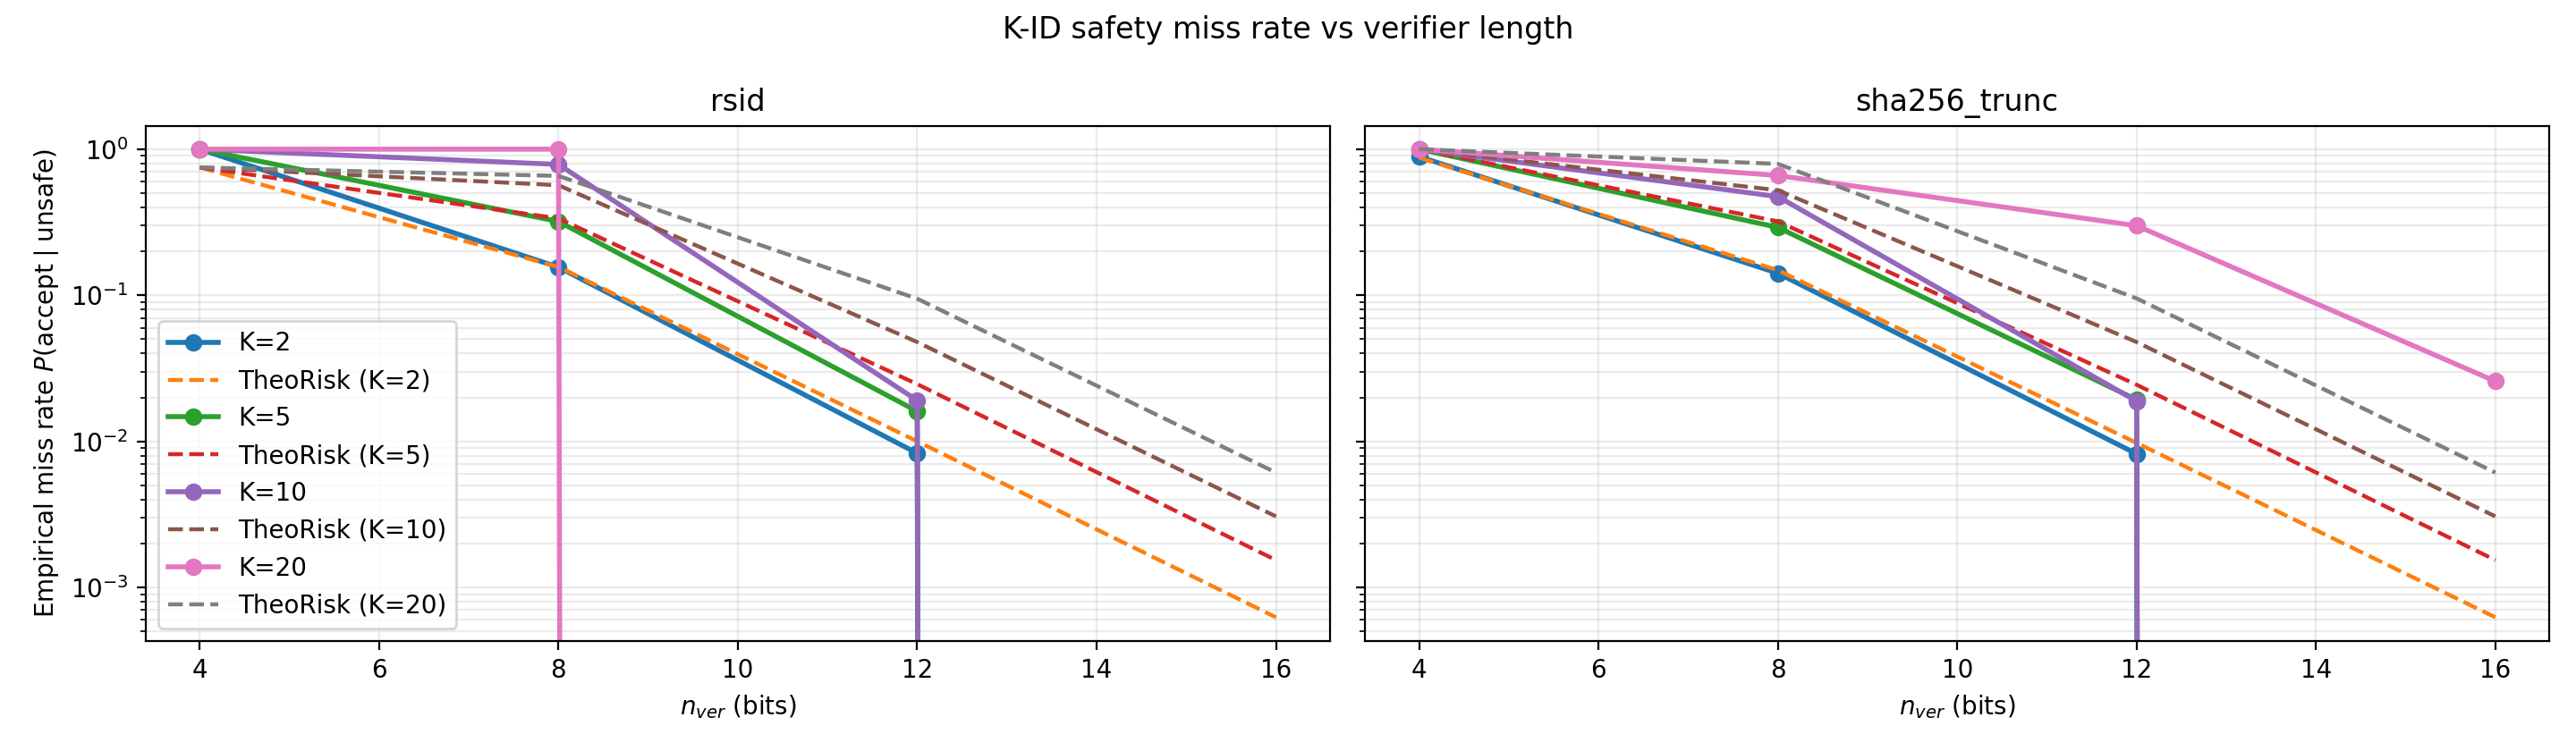
\includegraphics[width=\linewidth]{figures/plots/kid_sweep_uniform_both_miss_rate.png}
        \caption{Conditional miss rate (uniform error), by system.}
        \label{fig:kid_uniform_miss}
    \end{subfigure}\hfill
    \begin{subfigure}[t]{0.49\textwidth}
        \centering
        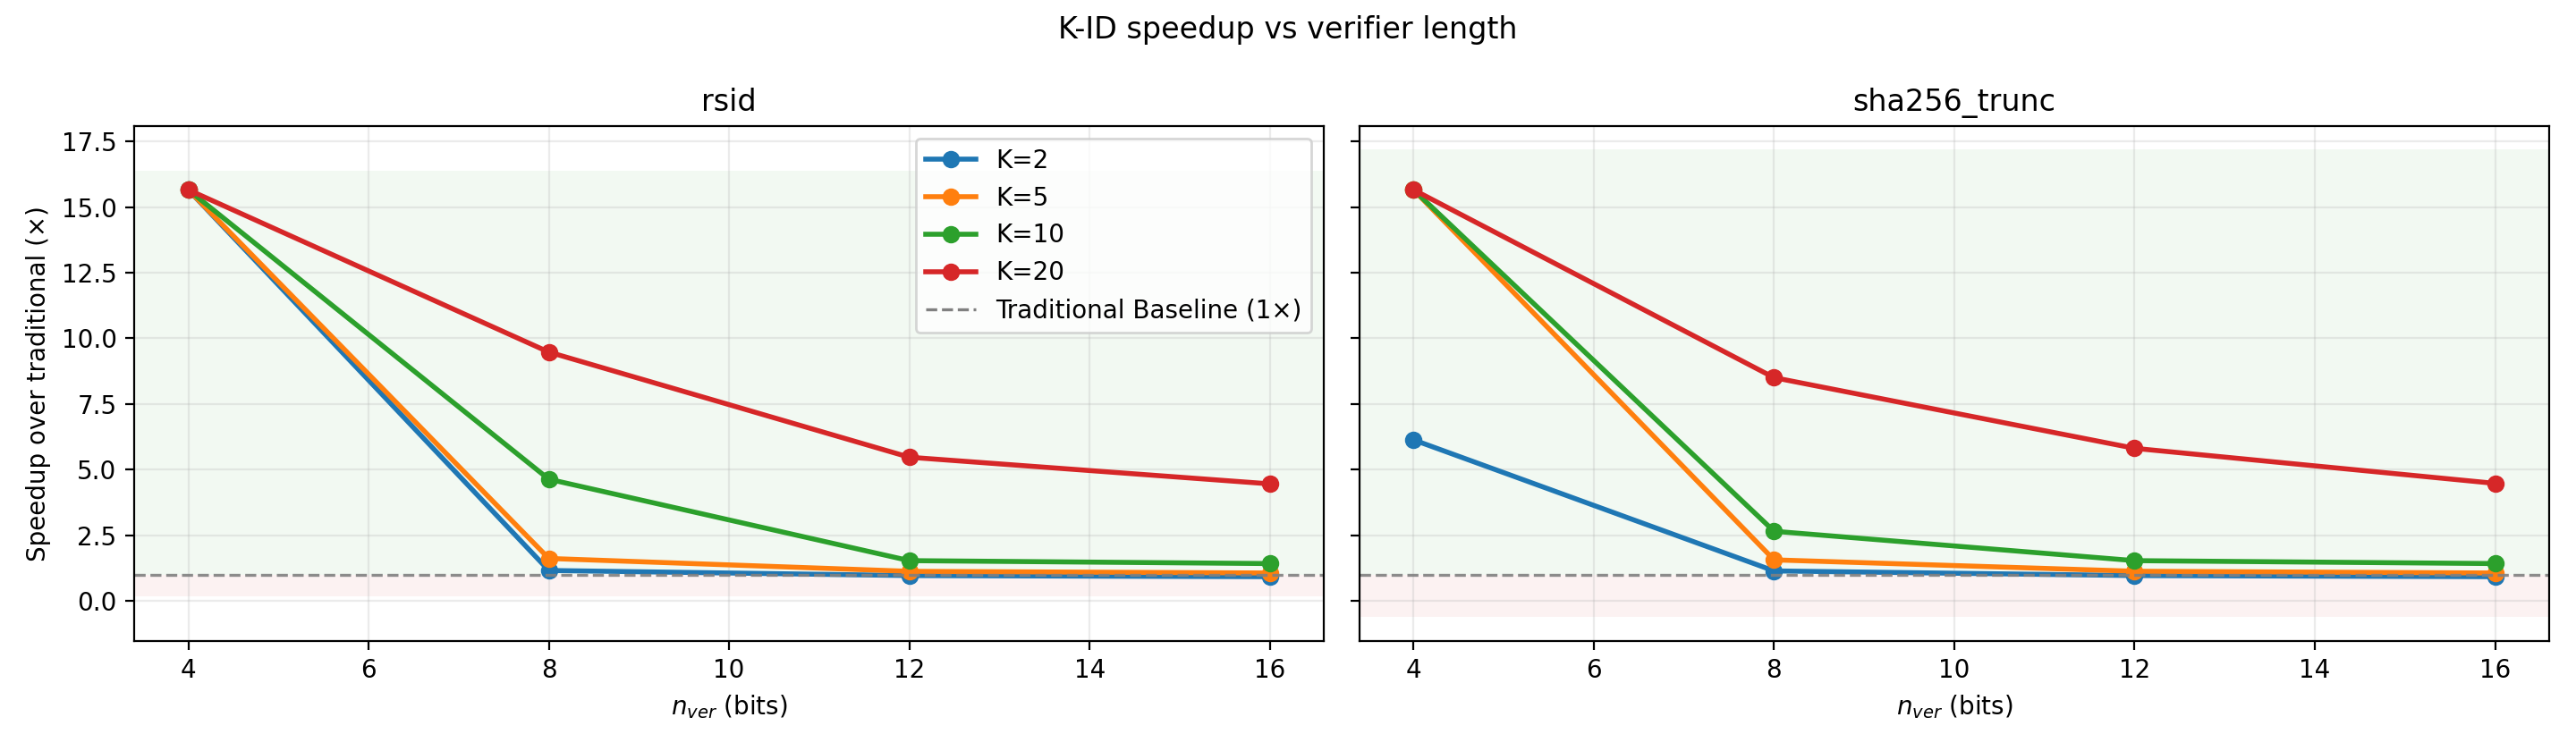
\includegraphics[width=\linewidth]{figures/plots/kid_sweep_uniform_both_speedup.png}
        \caption{Speedup (uniform error), by system.}
        \label{fig:kid_uniform_speedup}
    \end{subfigure}

    \vspace{0.6em}

    \begin{subfigure}[t]{0.49\textwidth}
        \centering
        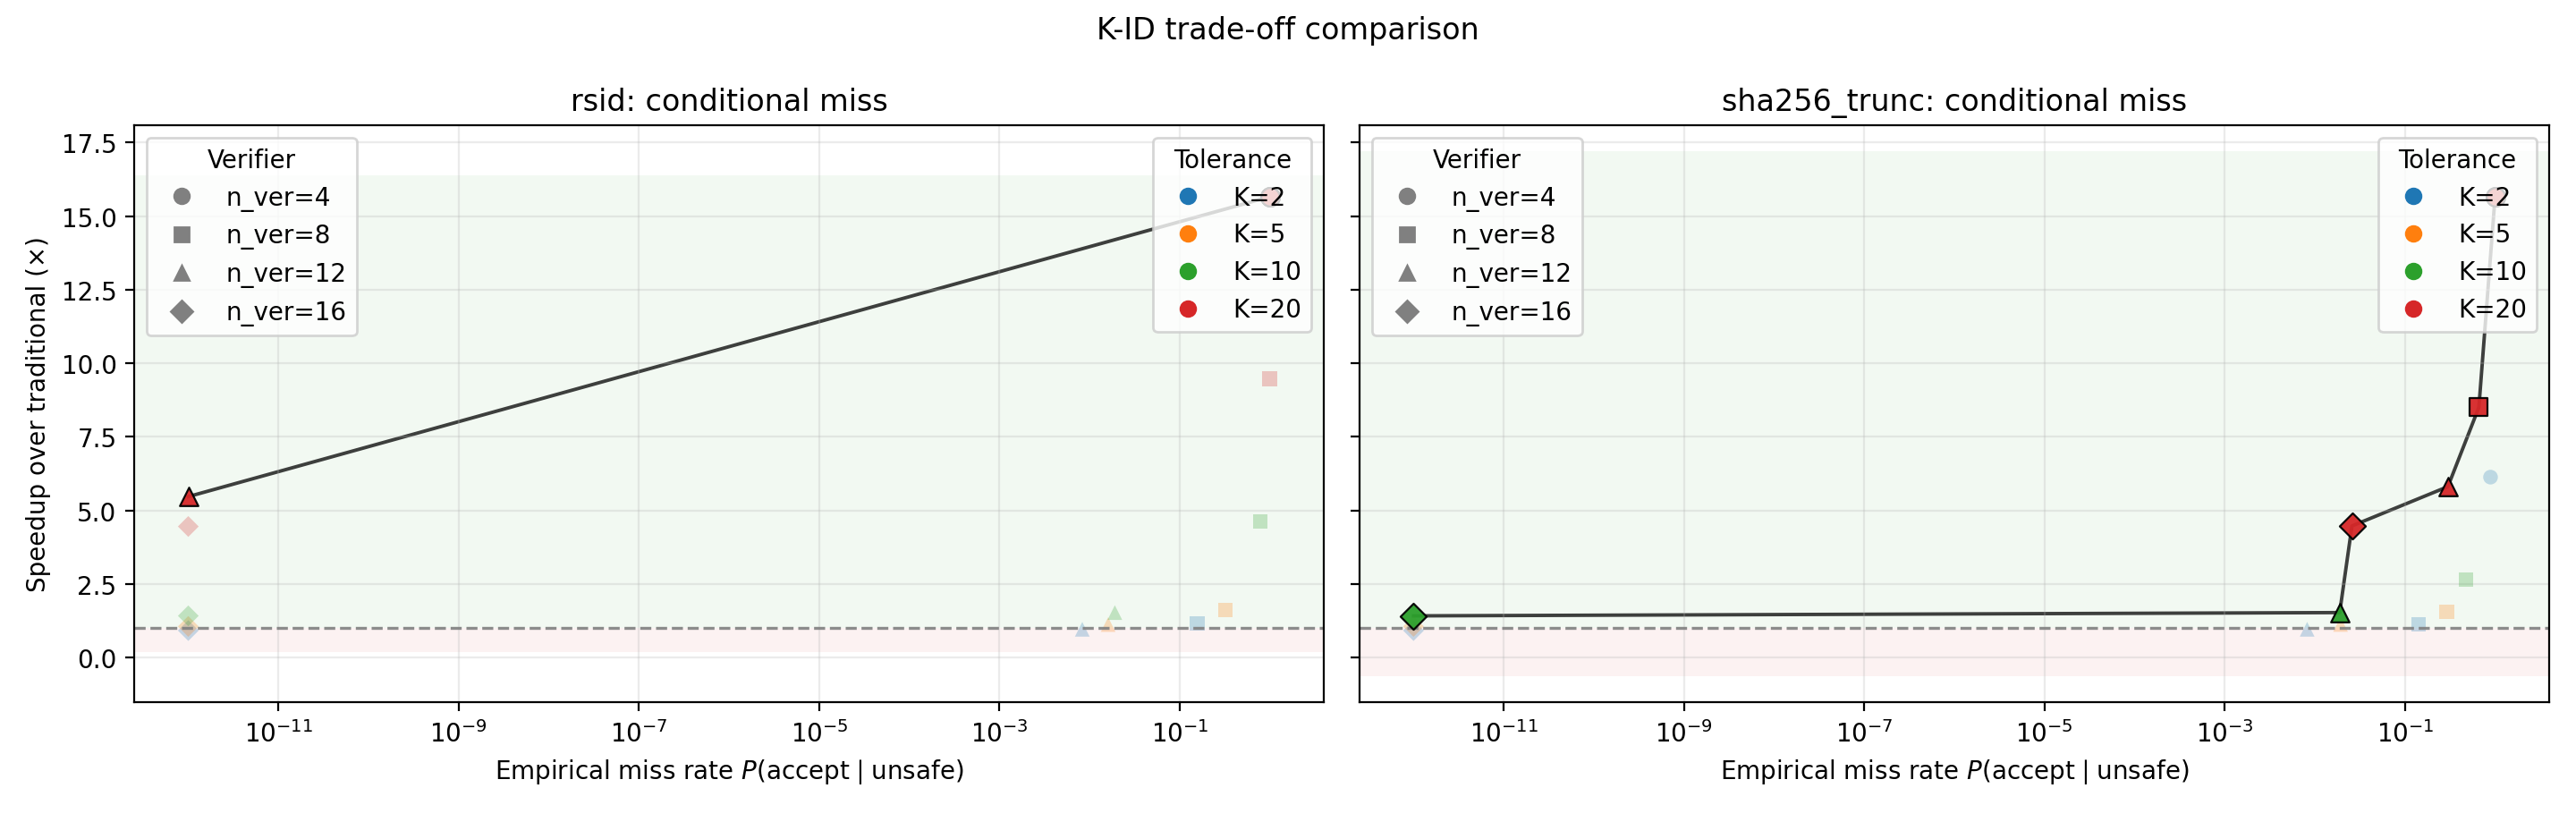
\includegraphics[width=\linewidth]{figures/plots/kid_sweep_uniform_both_pareto.png}
        \caption{Pareto trade-off: speedup vs. $P(\mathrm{accept}\mid\mathrm{unsafe})$.}
        \label{fig:kid_uniform_pareto}
    \end{subfigure}\hfill
    \begin{subfigure}[t]{0.49\textwidth}
        \centering
        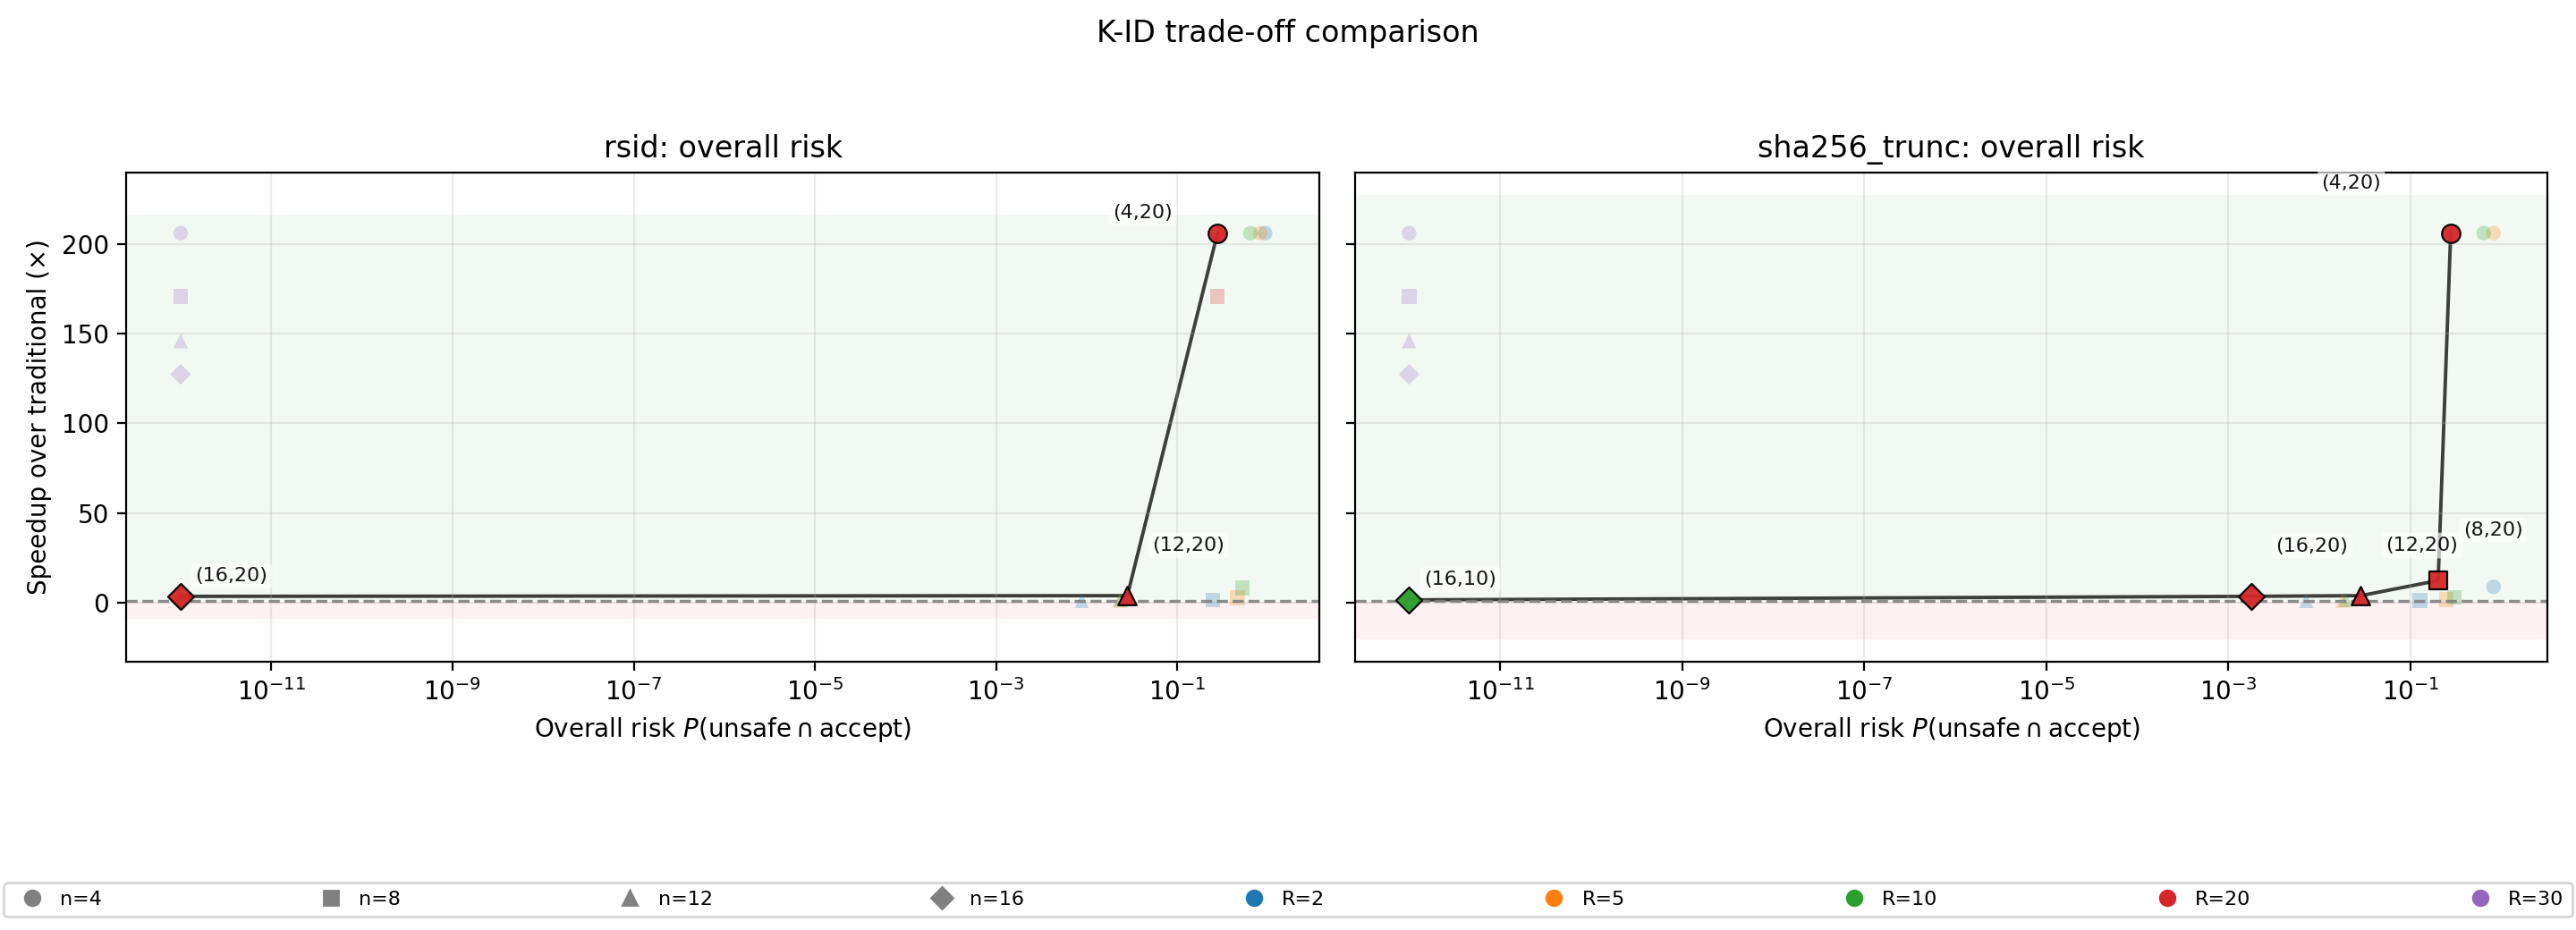
\includegraphics[width=\linewidth]{figures/plots/kid_sweep_uniform_both_pareto_overall_risk.png}
        \caption{Pareto trade-off: speedup vs. $P(\mathrm{unsafe}\cap\mathrm{accept})$.}
        \label{fig:kid_uniform_pareto_overall}
    \end{subfigure}

    \caption{K-ID sweep comparison of truncated SHA-256 vs. RS-ID under a uniform prediction error model ($n_{data}=96$ bits, $B=1$ Mbps).}
    \label{fig:kid_uniform_compare}
\end{figure}
\chapter{Conclusion and Future Work}
\label{ch:conclusion_and_future_work}
\label{sec:conclusion_and_future_work}

\section{Conclusion}
\label{sec:conclusion}

This thesis investigates \gls{id}-based synchronization for edge-based \glspl{dt} in bandwidth-constrained environments. Beyond reducing traffic volume, the \gls{id} mechanism can reduce end-to-end latency by replacing full payload transfer with \enquote{state verification}. The results support the following conclusions:

First, the \gls{id} protocol reduces the sensitivity of synchronization latency to state dimension in bandwidth-limited regimes. Experiments show that for $B < 1$ Mbps, \gls{id} yields lower end-to-end latency than full-state transmission. For high-dimensional sensor data such as \gls{lidar}, the additional encoding overhead is typically outweighed by reduced fallback transmission cost, improving freshness by avoiding unnecessary payload transfers.

Second, for the evaluated software stack, truncated hashing based on \glsentryshort{sha}-256 is typically a more practical engineering choice than algebraic coding via \gls{rsid} for edge deployments. The main driver is implementation efficiency: optimized \glsentryshort{sha}-256 backends achieve low and largely payload-independent encoding latency, whereas \gls{rsid} incurs higher computation that depends on the symbolization of the payload.

\gls{rsid} nevertheless remains relevant in two regimes. The first is high-integrity applications where rigorous mathematical error bounds are mandatory (i.e., a provable upper bound on failure probability under the stated modeling assumptions). The second is transmission-congested, fallback-heavy operation, where full-state recovery is triggered frequently and the resulting transmission delay dominates the end-to-end latency; in this regime, marginal compute-time differences between encoding mechanisms become comparatively less influential.

Third, \gls{kid} implements the shift from \enquote{bitwise exactness} to \enquote{semantic compliance}. The Pareto analysis shows that introducing a semantic tolerance radius $R$ allows the system to trade reduced verification frequency (and thus reduced fallback traffic) against increased acceptance-set size. In the evaluated sweeps, a moderate tolerance improves speedup substantially, while configurations with very loose tolerance (e.g., $R=30$) do not appear among the non-dominated points due to a saturation in speedup relative to the growth of the acceptance set.

As a practical guideline for the studied noise levels, $R\approx 20$ behaves as a knee point: further increases yield limited marginal speedup while reducing verifier selectivity. Here, selectivity refers to the verifier's physical sensitivity in distinguishing negligible drift (treated as semantically admissible) from critical deviations that should trigger recovery; as the acceptance set expands, a larger fraction of off-nominal states becomes indistinguishable from admissible noise at the verifier interface.

Fourth, the dynamic evaluation highlights time-correlated risk in the presence of probabilistic verification. Under random-walk drift, weaker verifiers can turn isolated collisions into persistent, undetected boundary breaches once $|E_t|>R$. The throughput analysis based on the \gls{sri} illustrates a two-tier control logic: the physical tolerance radius $R$ regulates the base synchronization rhythm (traffic sparsification), while verifier entropy $n_{ver}$ governs recovery reliability by suppressing collision-induced misses.

This also exposes an entropy-saturation feasibility constraint. Let $K\triangleq |\mathcal{A}_R|$ denote the acceptance-set size induced by the physical radius $R$ at quantization step $\Delta$ (e.g., in 1D, $K=2\lfloor R/\Delta\rfloor+1$). Under the accept-set approximation, the miss probability scales as $p_{miss}\approx K/2^{n_{ver}}$. If $K$ is comparable to or exceeds $2^{n_{ver}}$ (e.g., large $R$ at fine $\Delta$ with small $n_{ver}$), the verifier space becomes saturated and reliable detection cannot be guaranteed. Finally, the dynamic metrics show an inherent trade-off: increasing $R$ can reduce the typical duration of undetected intervals but increases the maximum physical drift accumulated during such events.

Overall, the evaluation quantifies the coupled trade-offs among computation, communication, and control fidelity, and yields design guidance for semantic synchronization policies in which tolerance radius $R$, acceptance-set size $K$, verifier entropy ($n_{ver}$), and quantization ($\Delta$) are selected jointly under bandwidth and safety constraints.

\section{Future Work}
\label{sec:future_work}

While this work has characterized the latency and reliability of \gls{kid}, several avenues remain to extend its theoretical depth and practical applicability in next-generation networks.

\subsection{Energy-Aware Identification Policies}
Current evaluations utilize traffic volume and latency as proxies for system efficiency. However, for battery-powered \gls{iot} devices, energy consumption is often the dominant constraint. Future work should explicitly model the energy--delay product, balancing the computational energy cost of hashing against the transmission energy cost of radio interfaces. By integrating the First-Order Radio Model~\cite{heinzelman2000energy} with real-time power profiling of edge hardware, we aim to derive an energy-optimal policy that dynamically adapts the tolerance radius $R$ (and thus the induced acceptance-set size $K$) and verifier length $n_{ver}$ based on the device's remaining battery life.

\subsection[Integration with 6G Physical Layer Security]{Integration with \glsentryshort{sixg} Physical Layer Security}
The current implementation relies on synchronized \glspl{prng}, which introduces a dependency on upper-layer clock synchronization protocols like \gls{ptp}. To align with the architecture of \gls{sixg} networks, future iterations will investigate the integration of \gls{plkg}. By exploiting the channel reciprocity in \gls{tdd} systems, the robot and the \gls{dt} can extract common randomness directly from the \gls{csi}. This approach would turn channel noise into a synchronization resource, eliminating the need for clock synchronization and enhancing robustness against timing attacks in harsh industrial environments.

\subsection{Scalability to Multi-Agent Systems}
This thesis focused on a single robot--\gls{dt} loop. However, industrial scenarios often involve swarms of robots sharing a physical workspace. A critical extension is the development of semantic multiple access schemes, where multiple robots superimpose their identification codes on a shared channel. Future work will explore algebraic constructions that allow the \gls{dt} to verify the aggregate safety of the swarm directly in the coded domain, checking for \enquote{Semantic Inter-Robot Collisions} without decoding individual states, thereby scaling the \gls{kid} paradigm to massive multi-agent systems.

\subsection[Predictive DTs and Adaptive K-ID]{Predictive \glsentryshortpl{dt} and Adaptive \glsentryshort{kid}}
The dynamic drift evaluation in this thesis uses a deliberately simple predictor (\gls{zoh}) to isolate protocol-induced effects. A natural next step is to integrate stronger predictors such as Kalman filtering or learned kinematic models, and to study how prediction quality reshapes both the masking risk (through the breach rate) and the collision risk (through the verification rate). In addition, future work should explore adaptive policies that tune $(R,n_{ver})$ online based on observed breach statistics and safety budgets, tightening the tolerance under persistent drift and relaxing it during stable operation to reduce bandwidth.

\subsection{Decoder Compute, Scheduling, and Quantization Sensitivity}
Beyond bandwidth and latency, practical deployments must also account for \glsentryshort{dt}-side compute and memory. Since the acceptance-set size scales as $K=|\mathcal{A}_R|\approx 2\lfloor R/\Delta\rfloor+1$ in 1D, a direct implementation precomputes $\mathcal{V}_R$ by hashing $\mathcal{O}(K)$ states per \glsentryshort{dt} update, and stores up to $|\mathcal{V}_R|\le K$ verifier codewords. Future work should therefore characterize end-to-end performance under explicit decoder compute constraints (e.g., bounded hash evaluations per tick), and study algorithmic accelerations (incremental updates, caching, \gls{gpu} offload).

In addition, the dynamic setting naturally suggests a scheduling-centric view: rather than only reporting per-tick risk, one can characterize the distribution of full-state update intervals (e.g., via \glspl{sri}, survival functions, and \gls{cdf} metrics) to answer questions like ``with 99\% probability, how long does the channel remain idle?'' Finally, because $\Delta$ is tied to sensor precision and \gls{dt} compute budget, a systematic sensitivity analysis over $\Delta$ is needed to guide robust configuration across heterogeneous sensing modalities.

\appendix
% ===============================================
%	The bibliography
% ===============================================
\printbibliography[heading=bibintoc]%
% ===============================================
%	The real appendix :D
% ===============================================
% !TEX root = thesis.tex
% ===============================================
% ===============================================
% 	LaTeX Chapter File - Appendix
% ===============================================
% ===============================================
\chapter{Appendix}

11
		
\end{document}
